\chapter{Experiment}

This chapter will describe the method of the experiment conducted in order to compare the gestures using the wristband to a VAS. For comparison a test was designed where the participants would be shown a stimuli and asked to input it using the gestures or a digital VAS. Two kinds of stimuli was used, an integer between zero and one hundred, or a box with a shade of grey between white and black based on the experiment by Matejka et al.\cite{grey}. Before describing the experiment further lets declare some terms for better clarification. As stated, there are three input methods:

\begin{enumerate}
\item The digital VAS. This is using a slider on the tablet. This input method will be referred to as \say{slider}
\item Using the wristband and the gesture of turning the wrist as described in Figure \ref{roll}. This input method will be referred to as \say{wrist}
\item Using the wristband and the gesture of raising the lower arm as described in Figure \ref{pitch}. This input method will be referred to as \say{arm}
\end{enumerate}

The two types of stimuli will be referred to as \say{num} and \say{grey} for the integer and shade of grey respectfully. With these three input methods and two stimuli a total of six different exercises must be conducted. The naming for each of these exercises is a combination of the input method and stimuli, e.g. turning your wrist to input a shade of grey will be referred to as \say{wrist\_grey}. All of the exercise's names can be seen in the top of Table \ref{latin}. The rest of this section will cover every aspect of this in more detail.

% % % % % % % % % % % % % % % % % % % % % % % %
% Participants % Participants % Participants %
% % % % % % % % % % % % % % % % % % % % % % % %
\section{Participants}
Twenty four (24) participants where chosen for this experiment. Since the experiment consist of six exercises a multiple of six was needed to ensure a minimal bias as explained later. Then based on the time frame for the experiment twenty four seemed to be a reasonable amount while being large enough to collect enough data. The participants volunteered their time and where not paid or in other ways obligated to participate. All of the participants were either from The Department of Applied Mathematics and Computer Science at DTU or the authors colleagues at IBM, thus most of the participants had above average technical experience, but based on the survey conducted after the experiment (Appendix \ref{survey}) 42\% had not any prior experience with wearable devices.

Out of the twenty four participants 18 where men and 6 where female. The mean age was 27.83 and the median age was 26.5, both age and gender distribution can be seen in Figure \ref{age_gender}.

\begin{figure}[h!]
    \centering
    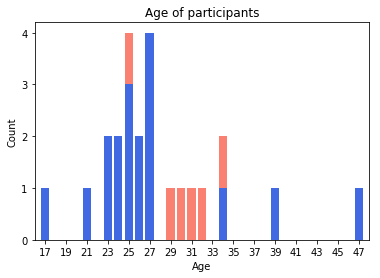
\includegraphics[width=.6\textwidth]{figures/age_gender.png}
    \caption{Age and gender distribution of the 24 participants: 18 males in blue \& 6 females in red}
    \label{age_gender}
\end{figure}



% % % % % % % % % % % % % % % % % % %
% Apparatus % Apparatus % Apparatus %
% % % % % % % % % % % % % % % % % % %
\section{Apparatus}
\subsection{Essential Hardware}
For the experiment three pieces of hardware was used:
\begin{enumerate}
\item MetaMotionR by mbientlab\cite{mbient} as the wristband device for registering input from the participant using the gestures
\item Samsung Galaxy Tab S2\cite{samsung}, this tablet run the app developed for the experimenting, keeping track of exercises, showing stimuli, collecting input from the participant, saving the data etc. Much more detail about this is this section
\item A computer used to fill in the survey after the experiment. In the experiment a MacBook Pro 13 inch model was used, although the computer used isn't important
\end{enumerate}

\subsection{App}
The app created for the experiment is built upon the same code as the companion app described in Chapter \ref{implementation}, but changed to fit the experiment. Has three main functions: Settings, Train and Experiment as seen in Figure \ref{app_main}. The settings is for configuring the experiment and exporting or deleting the collected data as seen in Figure \ref{app_settings}. Two variables can be changed that has influence on the experiment, the first is the \say{Number of stimuli}, this value will change the number of stimuli the participant has to rate for each exercise, the number of stimuli can be changed in steps of five. The \say{Next Subject ID} will change the ID used to identify each subject in the data. The order of exercises for the participant is bases on this value. Both of these settings should not be changed though out the experiment, so that the participant's IDs will be in sequential order and that they have the same amount of stimuli for each exercise. For this experiment the number of stimuli was set two 20 based on pilots tests.

Beside these two settings there is the option to \say{Toggle back button}, when this option is enabled a \say{Back} button will appear on any screen in the app, and when pressed will go back to the main screen. This option is purely for debugging allowing one two go back to the main screen at any point, during the experiment this options should be disabled. 

The last actions on this screen is to export and delete data. There are two options to export the date: \say{Move data} and \say{Email data}, the first will simply copy the collected data from the internal storage of the app to the external storage on the tablet so it can be accessed by any file manager. The later will also copy the date to external storage, but it will create an intent to email the data which will start the default email app and attach the data. \say{Delete data} will delete the collected data from internal storage, a confirmation prompt will appear first to prevent accidental deletion. Whenever the main or setting screen is accessed, the current battery percentage from the MetaMotionR is displayed on the screen, keeping an eye on this prevent the wristband to run out of power in the middle of the experiment.

\begin{figure}[h!]
\centering
\begin{minipage}{.55\textwidth}
  \centering
  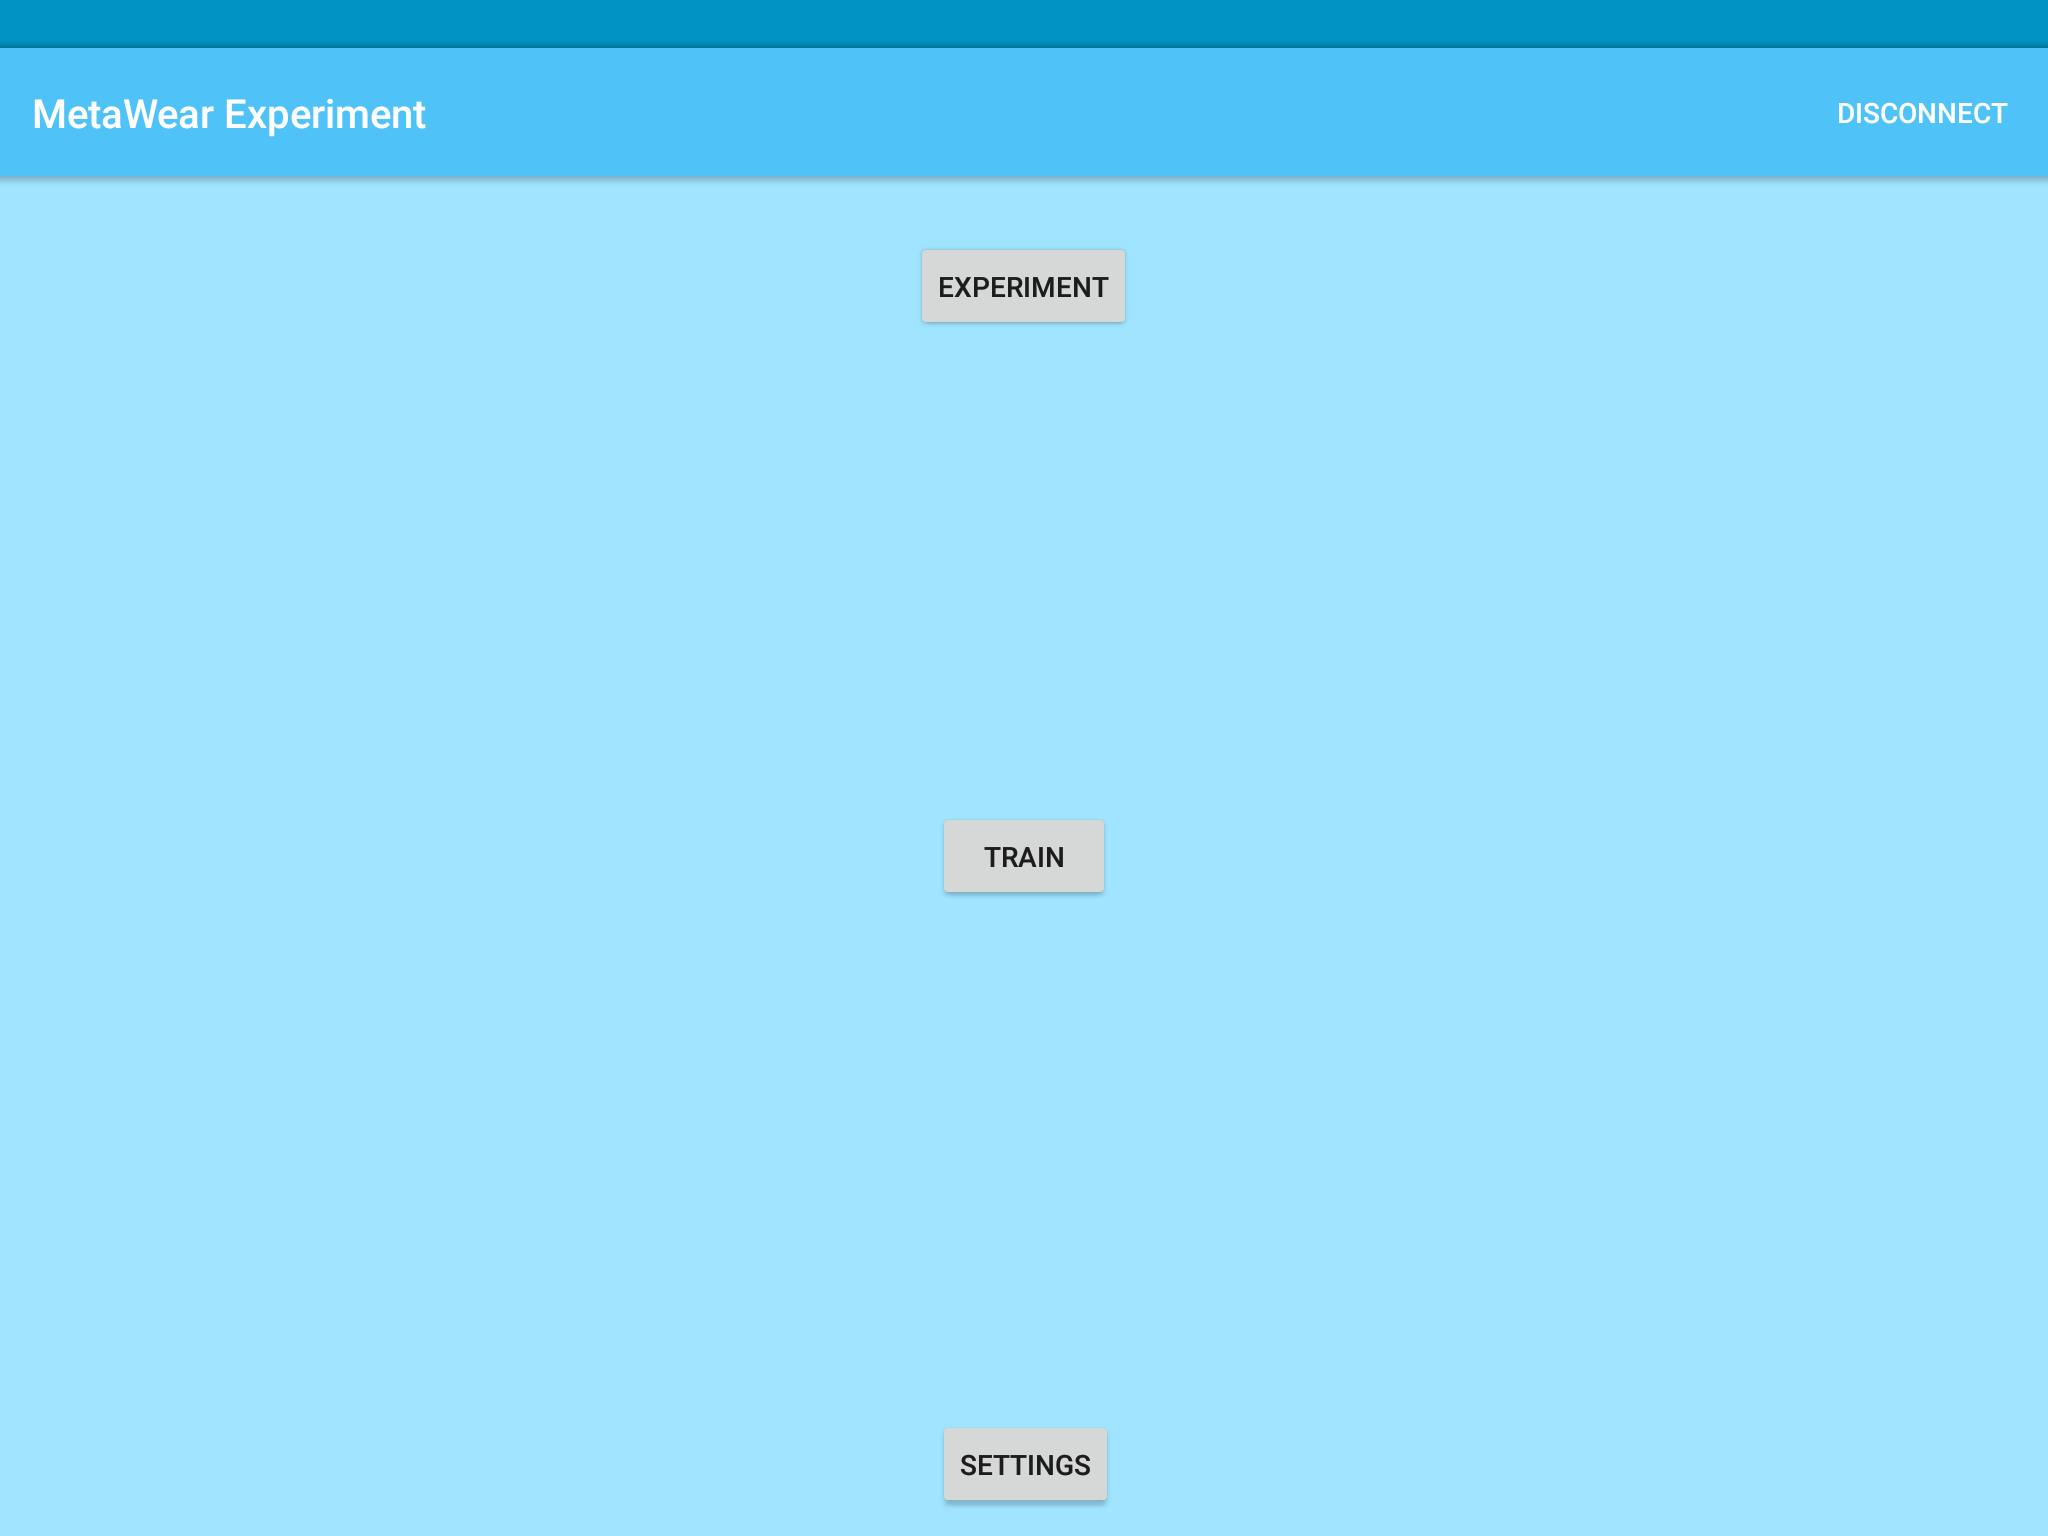
\includegraphics[width=0.95\linewidth]{figures/tablet_screen0.png}
  \captionof{figure}{Experiment app main screen}
  \label{app_main}
\end{minipage}%
\begin{minipage}{.55\textwidth}
  \centering
  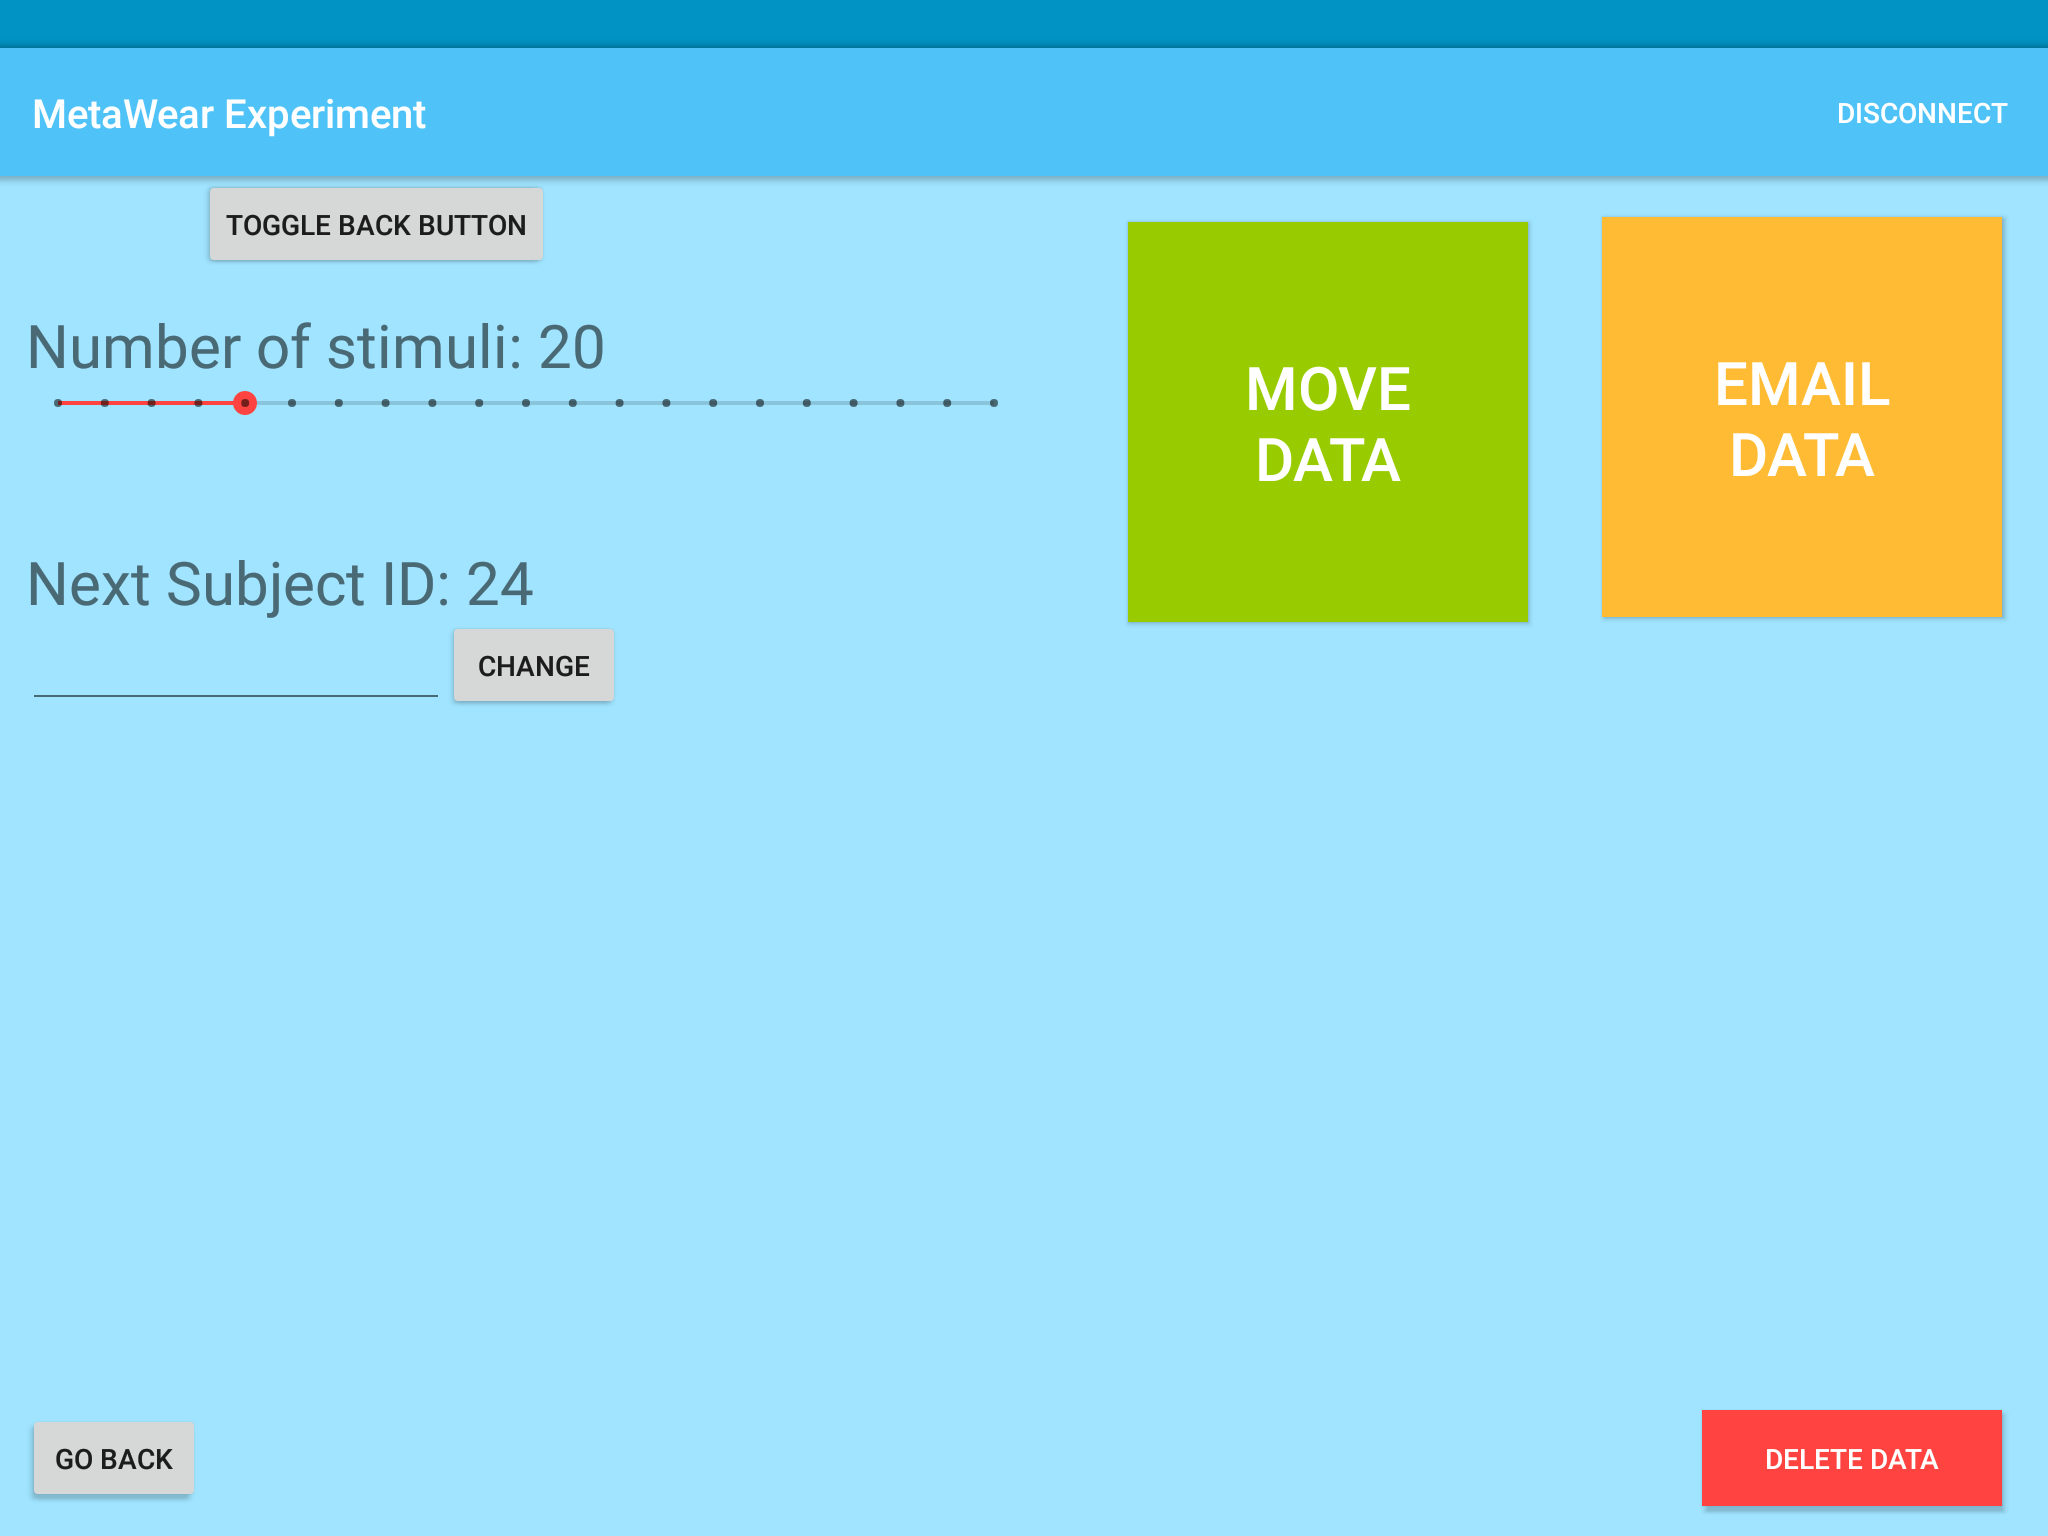
\includegraphics[width=0.95\linewidth]{figures/tablet_screen1.png}
  \captionof{figure}{Settings screen}
  \label{app_settings}
\end{minipage}
\end{figure}

The train screen is made to let the participant practice using the wristband device and get a feeling of the scale. When this screen is activated the wristband will be programmed similar as explained in Chapter \ref{implementation}, when the button is pressed it will read the orientation from its IMU and transmit it to the tablet. The light will flash and vibration motor will do a short pulse to provide feedback. The difference between the previous described implementation and the programming for the experiment is that instead of logging the data for later export, it will transmit it instantly. When the orientation data is received by the app it will map the Euler angles to a 0-10 scale and display the result. The mapping is dependant on the toggle switch, if the switch is in the \say{Hand} position as in Figure \ref{app_train_wrist} the mapping will depend on the roll angle and if the switch is in the \say{Arm} position as in Figure \ref{app_train_arm} the mapping will depend on the pitch angle. This of course correspond to the gestures described in Figure \ref{roll} and \ref{pitch}. As mentioned the roll angle will always be between -90º and 90º depending if the orientation clock or counter clock wise compared to 0º (horizontal). To map the values to a 0-10 scale the absolute value is divided by 9, e.g 90º/-90º will become 10, 45º/-45º will become 5, 25º/-25º will become 2.7778 etc. Mathematically this can be expressed with this function where \emph{sv} is the scaled value from 0-10 and \emph{ra} is the Euler angle for the roll axis:
\begin{center}
$sv\left ( ra \right ) = \frac{abs\left (ra\right )}{9}$
\end{center}

A consequence of this mapping is that if the participant turn the wristband pass the vertical position the scaled value will begin to decrease. This means that the participant won't achieve a 10 rating simply by turning the wrist way beyond the vertical position. A different solution could be made to detect when the wristband pass the vertical position and set the scaled value at 10. It can be debated as to which solution is the greater, but by letting the scaled value decrease will force the participant to get a better sense of the scale and won't allow \say{lazy} responses.

Mapping the pitch angle is a little more complicated, since the roll value will be between -180º and 180º. The soltuion is to create a function that maps the value differently depending if the absolute pitch angle is greater than 90, basically first mapping the -180º to 180º range down to a -90º to 90º degree range, and then mapping it to the scaled value. This function will express this where \emph{sv} is the scaled value from 0-10 and \emph{pa} is the Euler angle for the pitch axis:
\begin{center}
$sv\left ( pa \right ) = \left\{\begin{matrix}
\frac{90-\left ( abs\left ( pa \right )-90 \right )}{9} & if\ pa> 90 \\ 
\frac{abs\left ( pa \right )}{9} & otherwise
\end{matrix}\right.$
\end{center}

This mapping has the same property as explained before, where if the pitch angle goes pass the vertical position the scaled value will decrease.




\begin{figure}[h!]
\centering
\begin{minipage}{.55\textwidth}
  \centering
  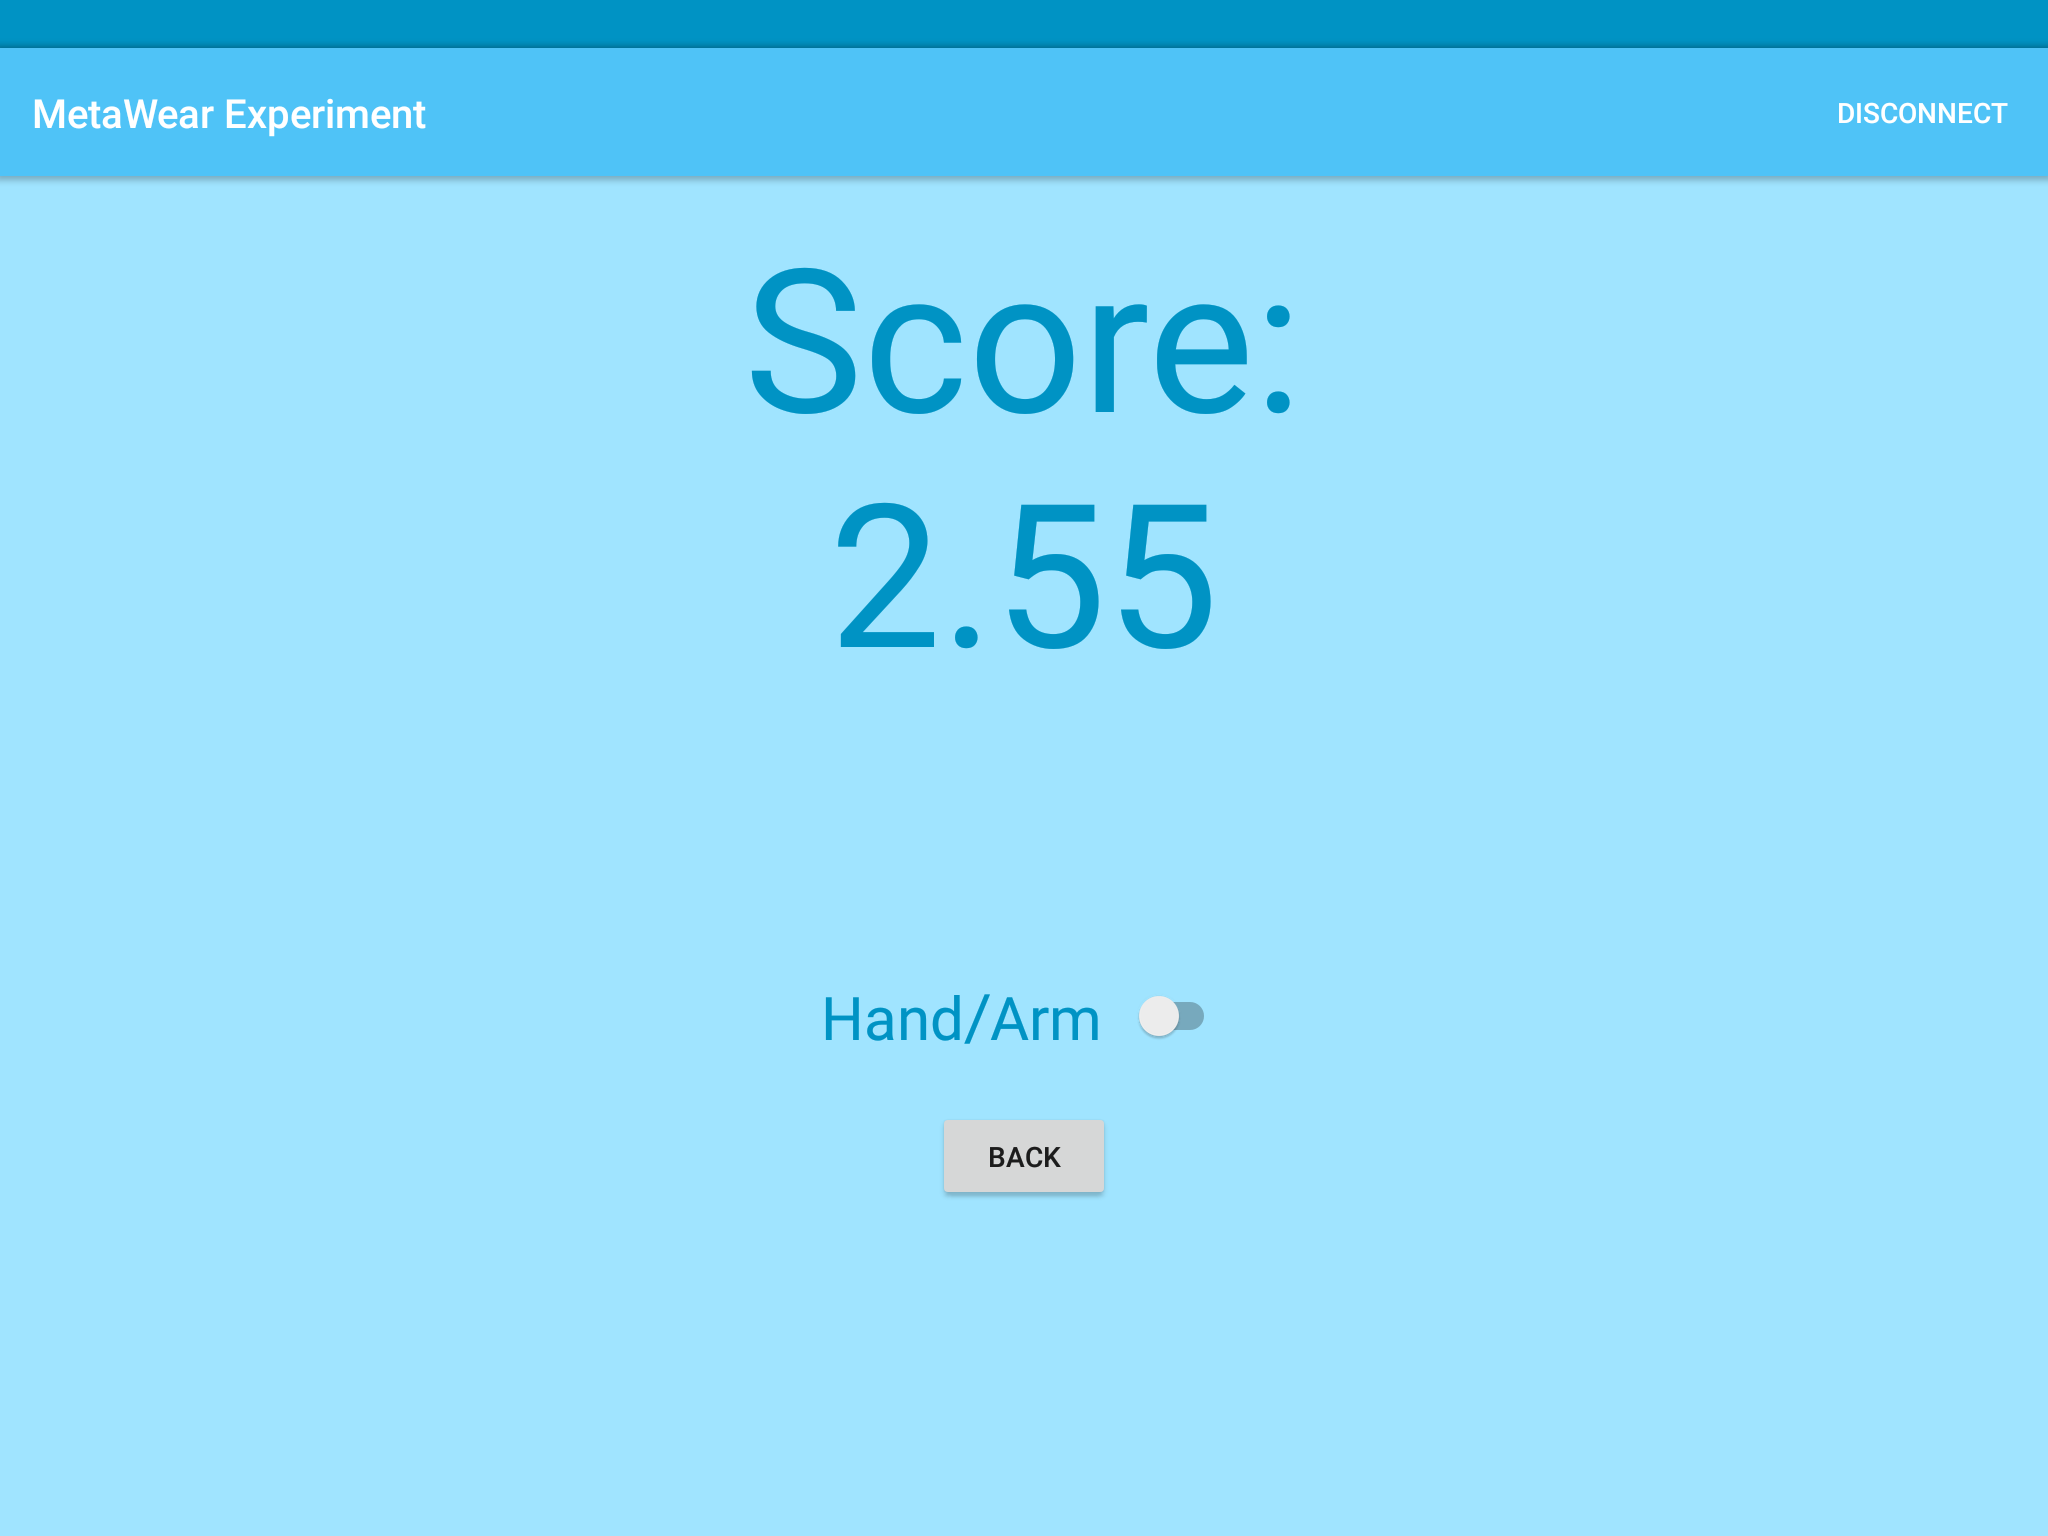
\includegraphics[width=0.95\linewidth]{figures/tablet_screen3.png}
  \captionof{figure}{Train screen hand (wrist) mode}
  \label{app_train_wrist}
\end{minipage}%
\begin{minipage}{.55\textwidth}
  \centering
  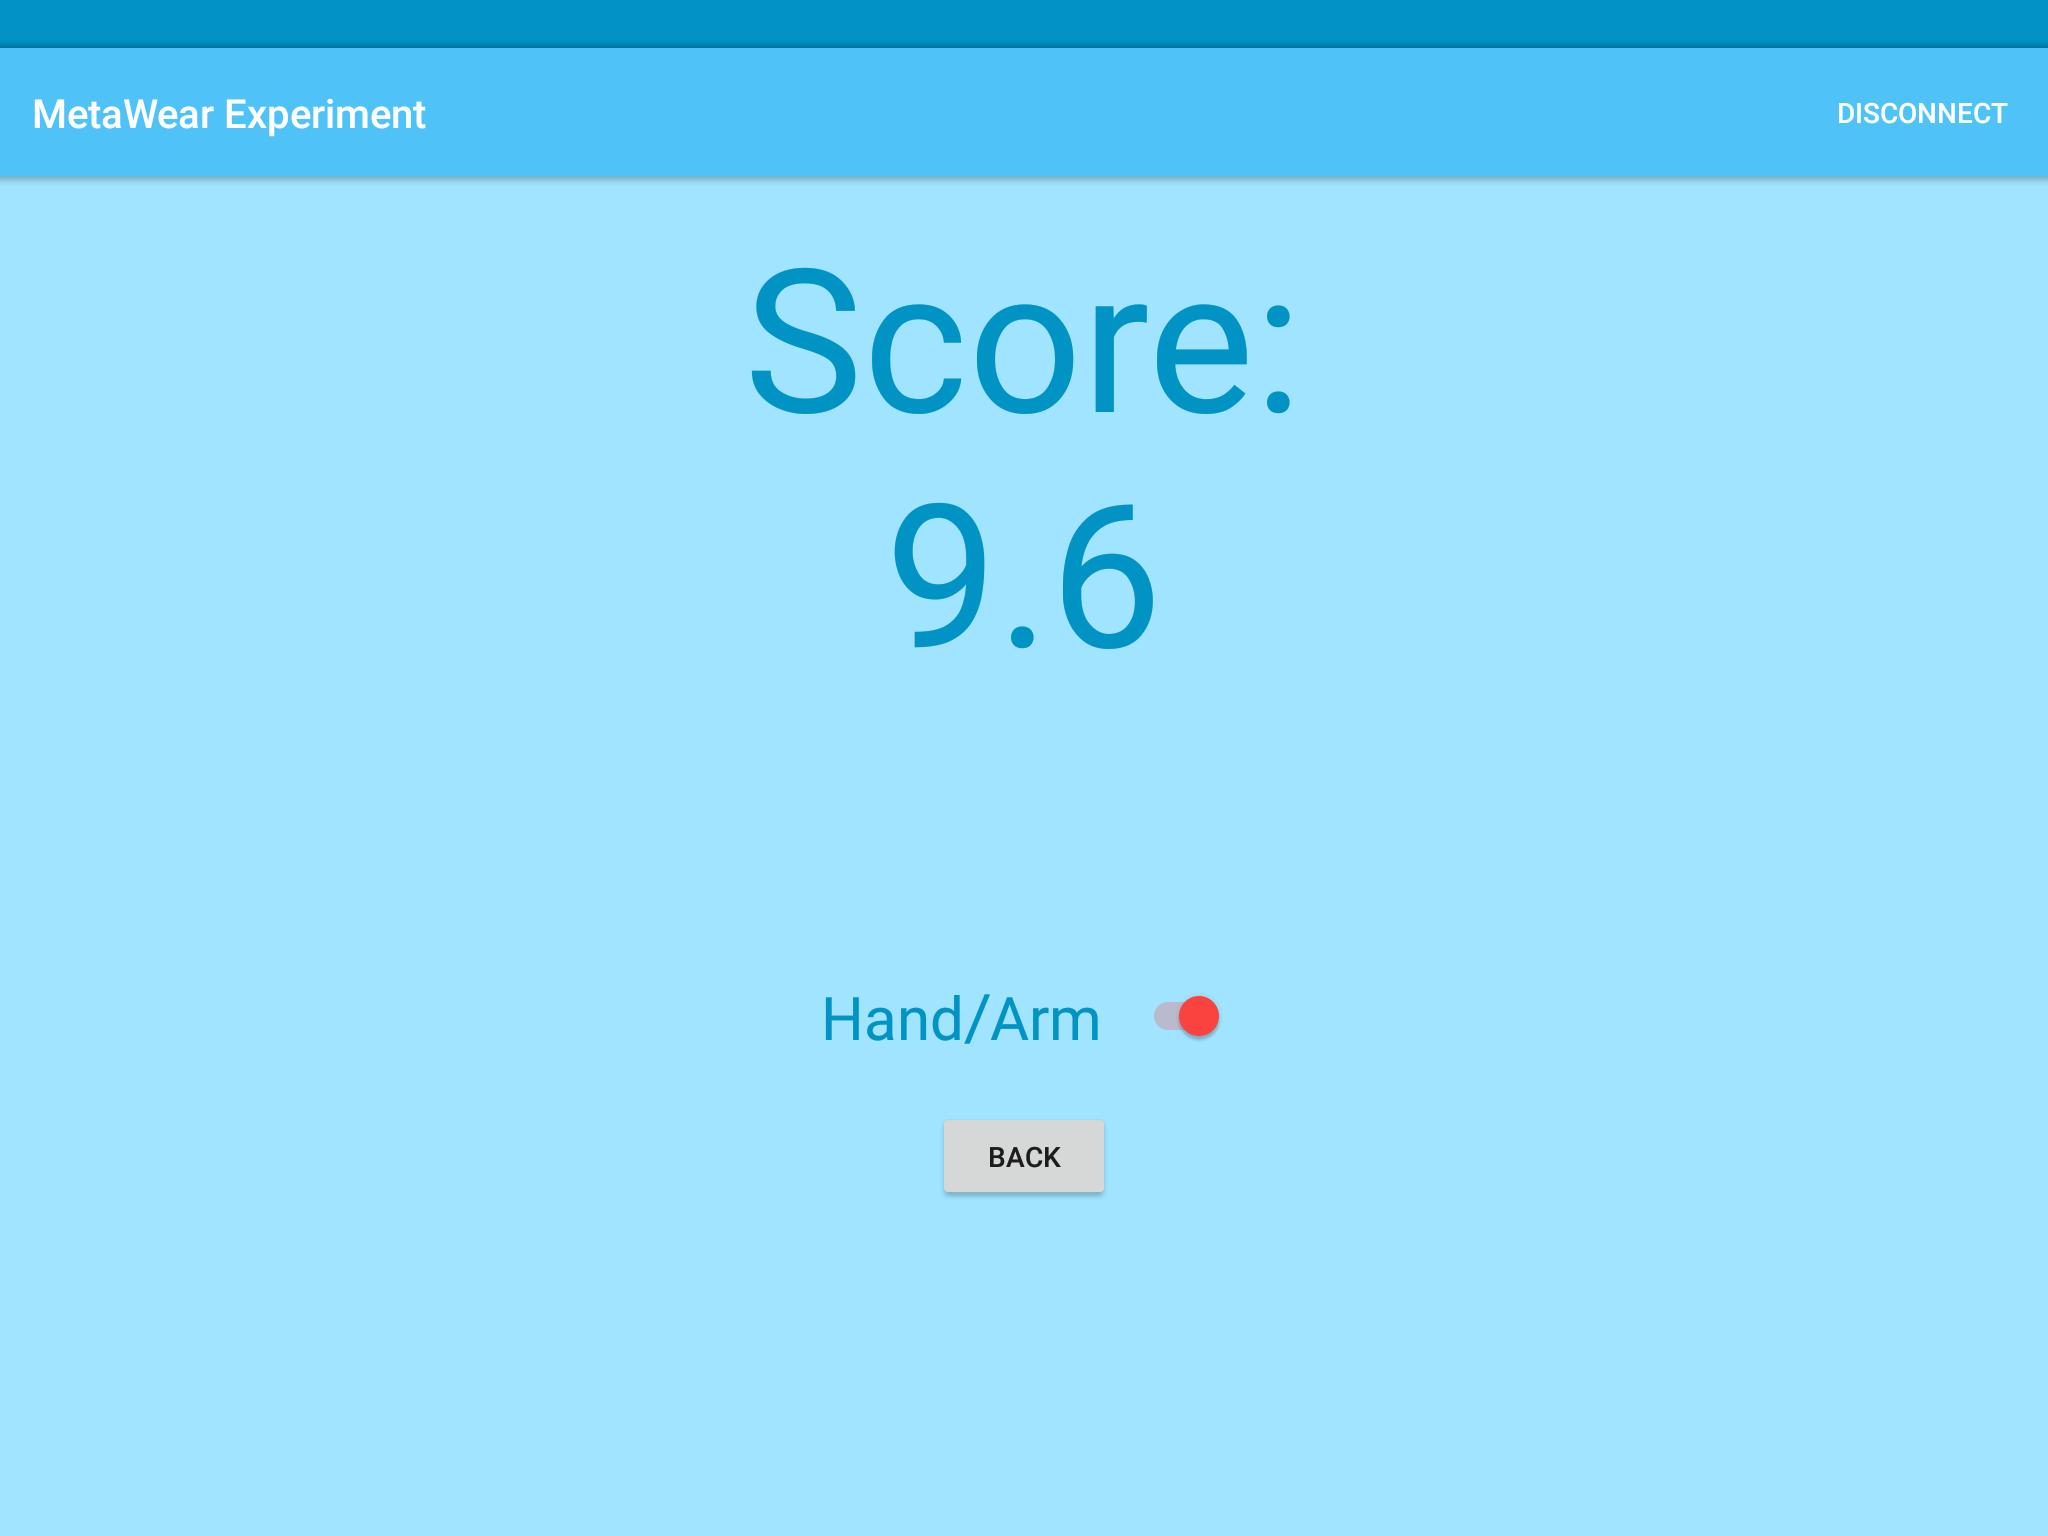
\includegraphics[width=0.95\linewidth]{figures/tablet_screen4.png}
  \captionof{figure}{Train screen arm mode}
  \label{app_train_arm}
\end{minipage}
\end{figure}

The last screen is the experiment itself, this is the most complicated screen and consist of many \say{sub screens}. Before the experiment begin a screen for inputting the gender and age of the participant is presented as seen in Figure \ref{app_ex_start}. In the top right the assigned ID for the participant is showed, this is just for confirmation and to be used in the survey after the experiment (so the survey and experiment data can be synchronized if needed). Once the \say{Start} button is pressed the experiment will begin. As mentioned the experiment consist of six exercises and the order of these is dependent on Table \ref{latin}. Before each exercise an explanation screen will show, this screen will have some text to explain the task of the exercise and a short GIF that illustrates it. The text will stay on top during the whole exercise. This screen purpose is to make sure the participant is sure of what task they are required to do, the participant will have gotten instructions beforehand, so this screen is just reassure them. Three of the six explanation screens can be seen in Figure \ref{app_slider_explain}, \ref{app_arm_explain} and \ref{app_wrist_explain}.

\begin{figure}[h!]
\centering
\begin{minipage}{.55\textwidth}
  \centering
  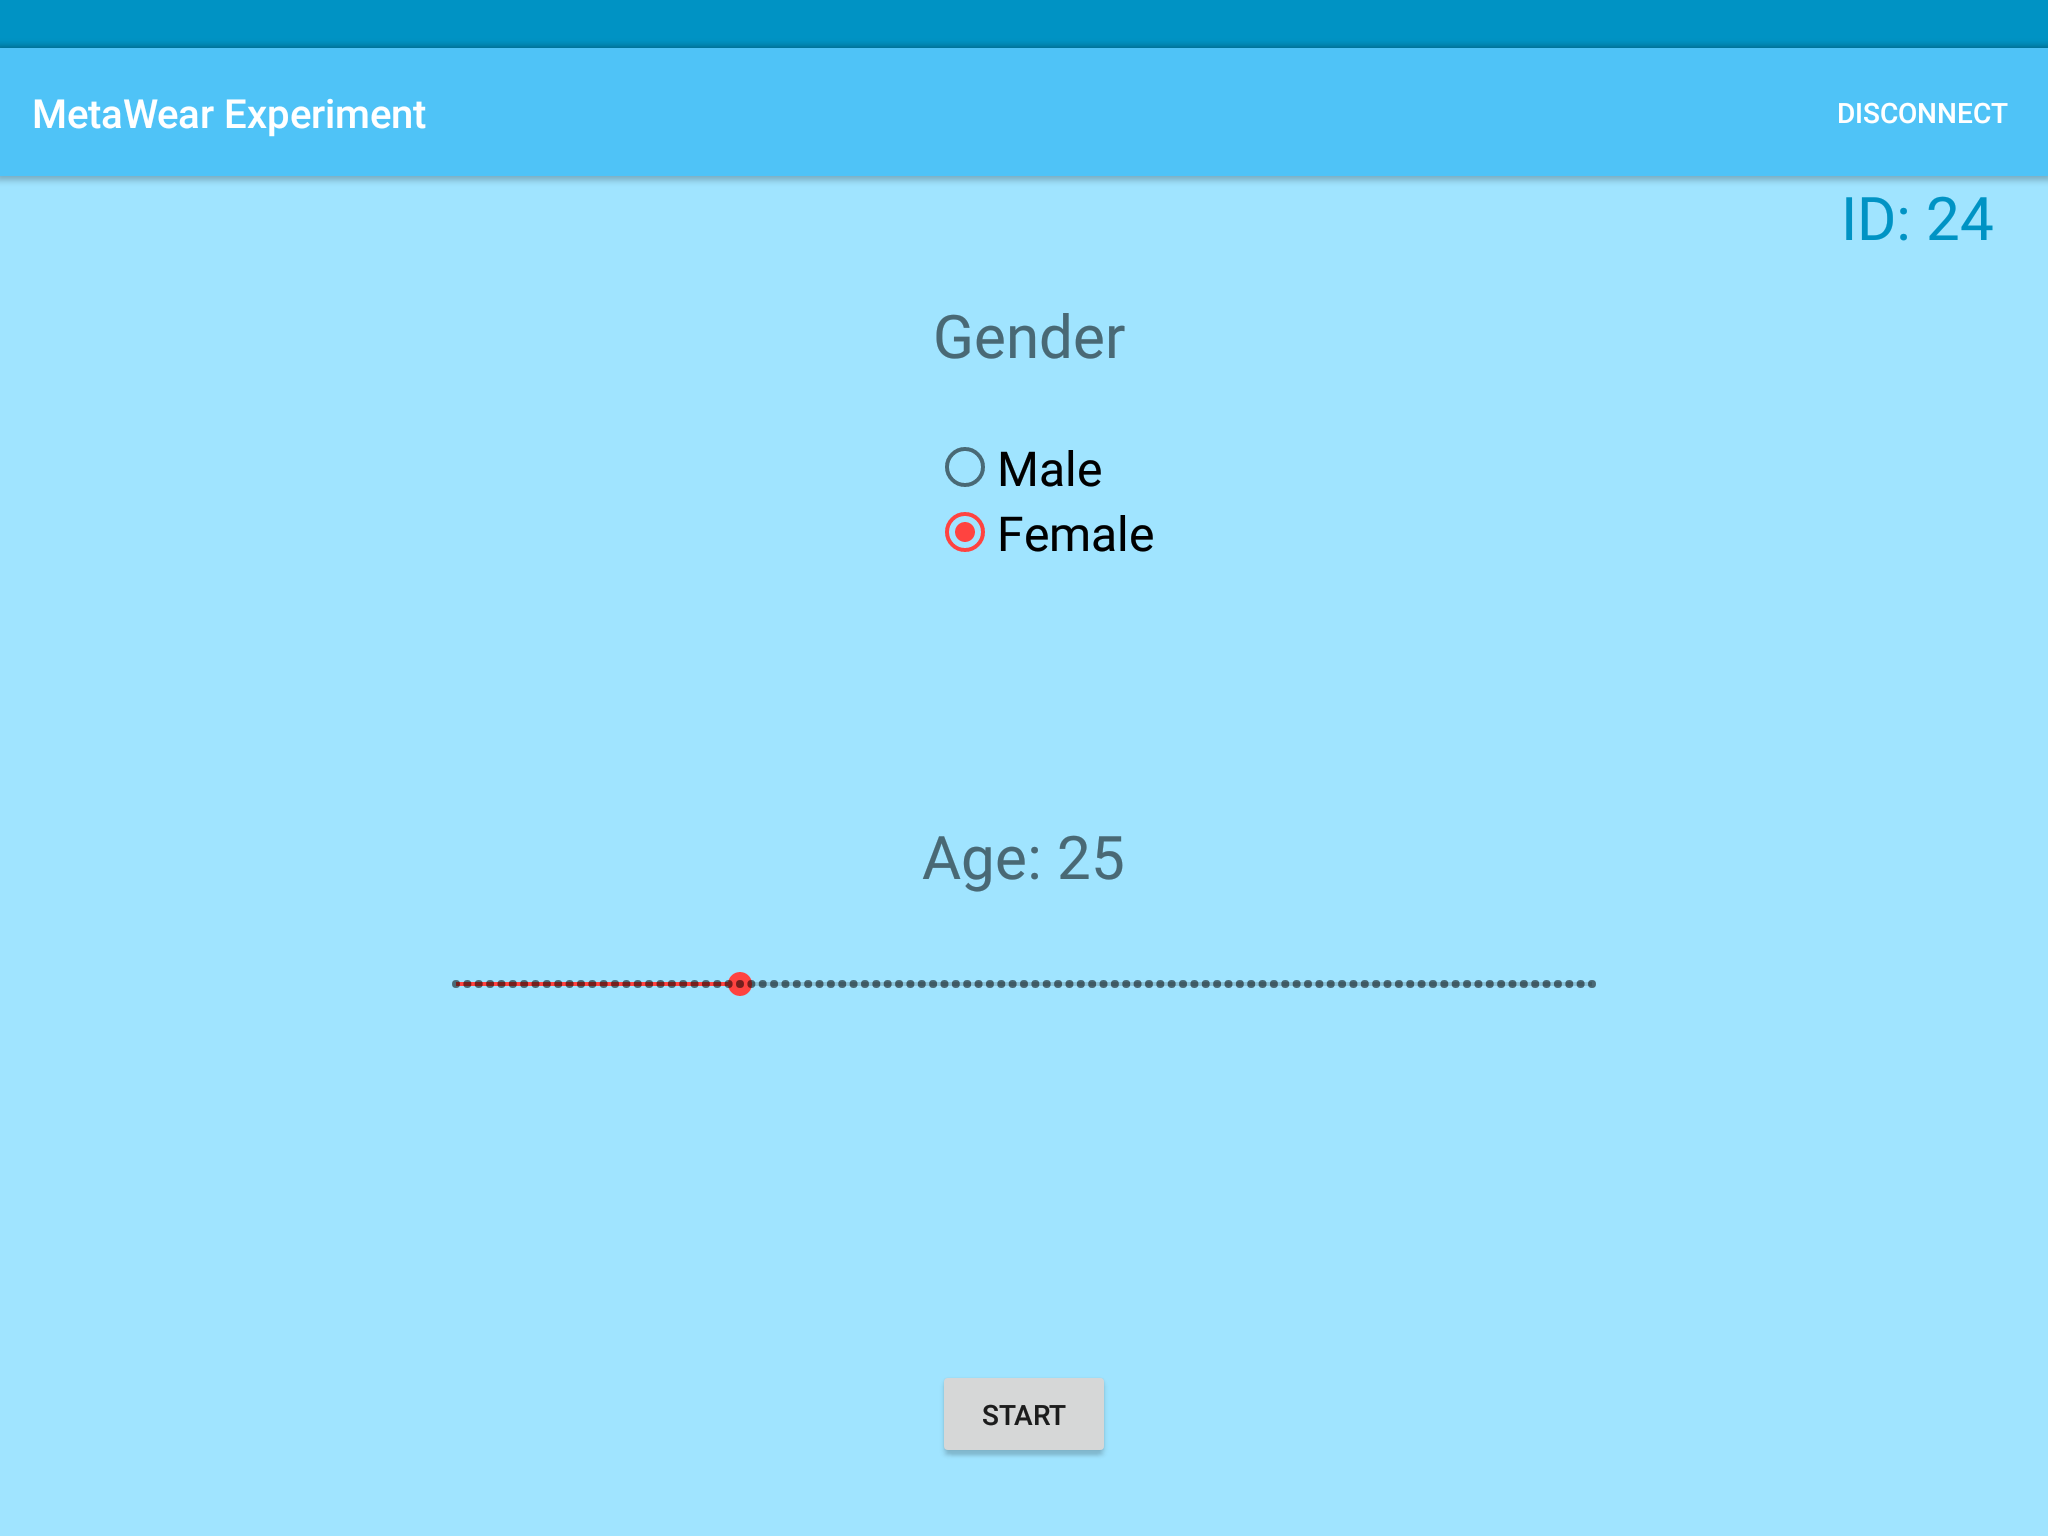
\includegraphics[width=0.95\linewidth]{figures/tablet_screen5.png}
  \captionof{figure}{Experiment start screen}
  \label{app_ex_start}
\end{minipage}%
\begin{minipage}{.55\textwidth}
  \centering
  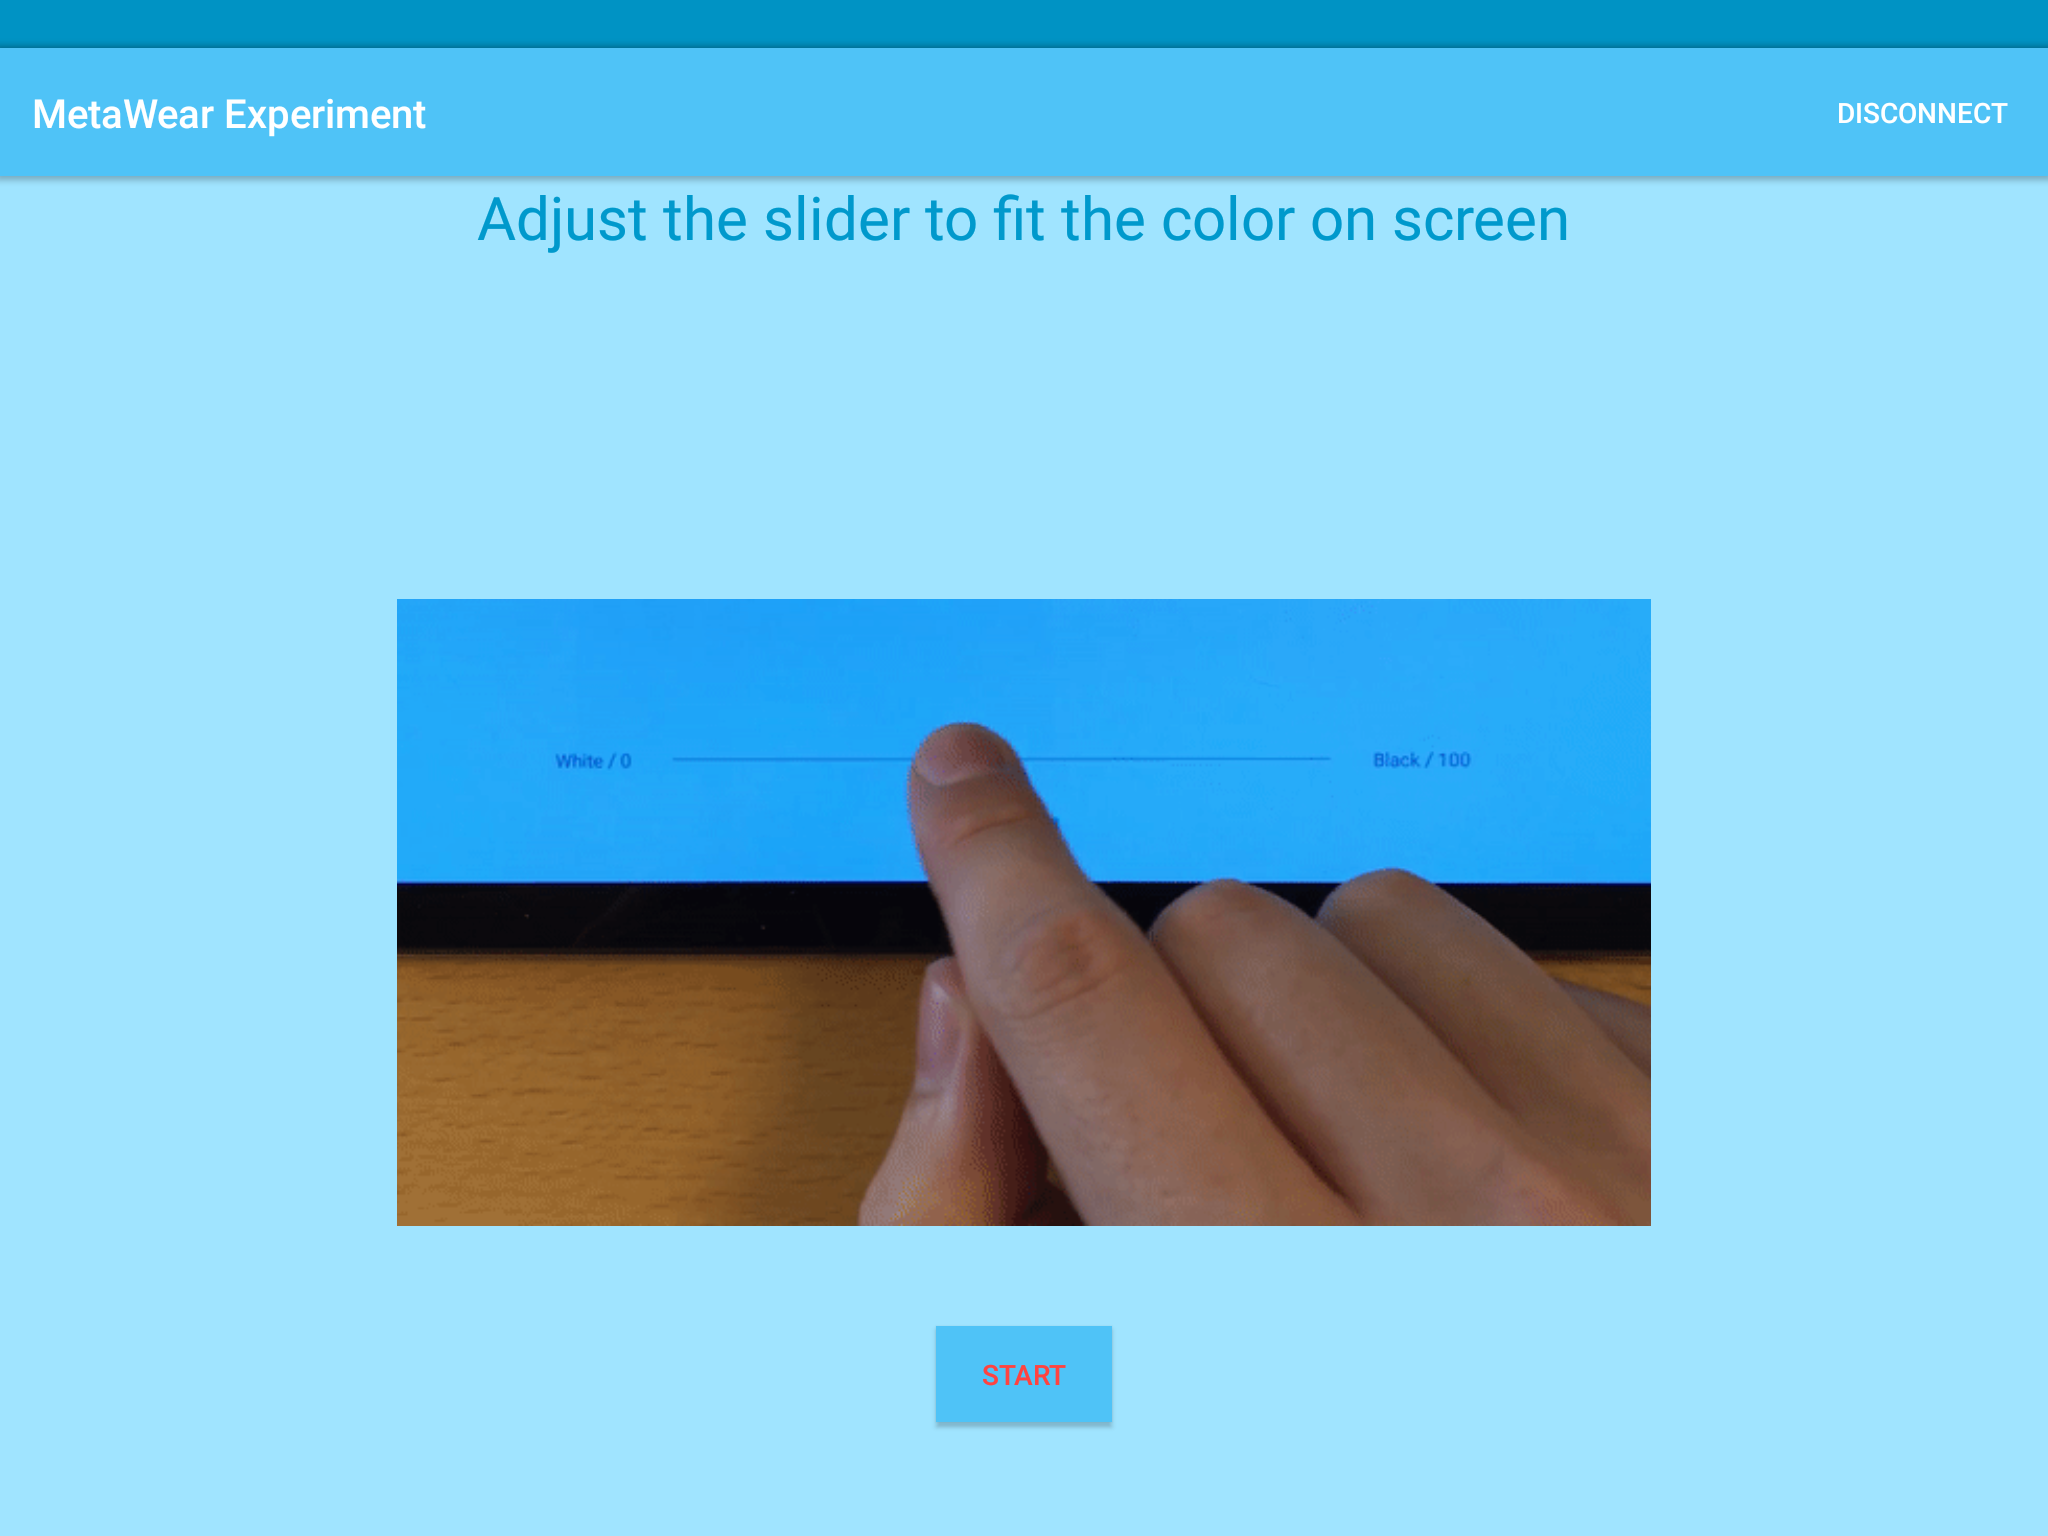
\includegraphics[width=0.95\linewidth]{figures/tablet_screen6.png}
  \captionof{figure}{slider\_grey explanation screen}
  \label{app_slider_explain}
\end{minipage}
\end{figure}

\begin{figure}[h!]
\centering
\begin{minipage}{.55\textwidth}
  \centering
  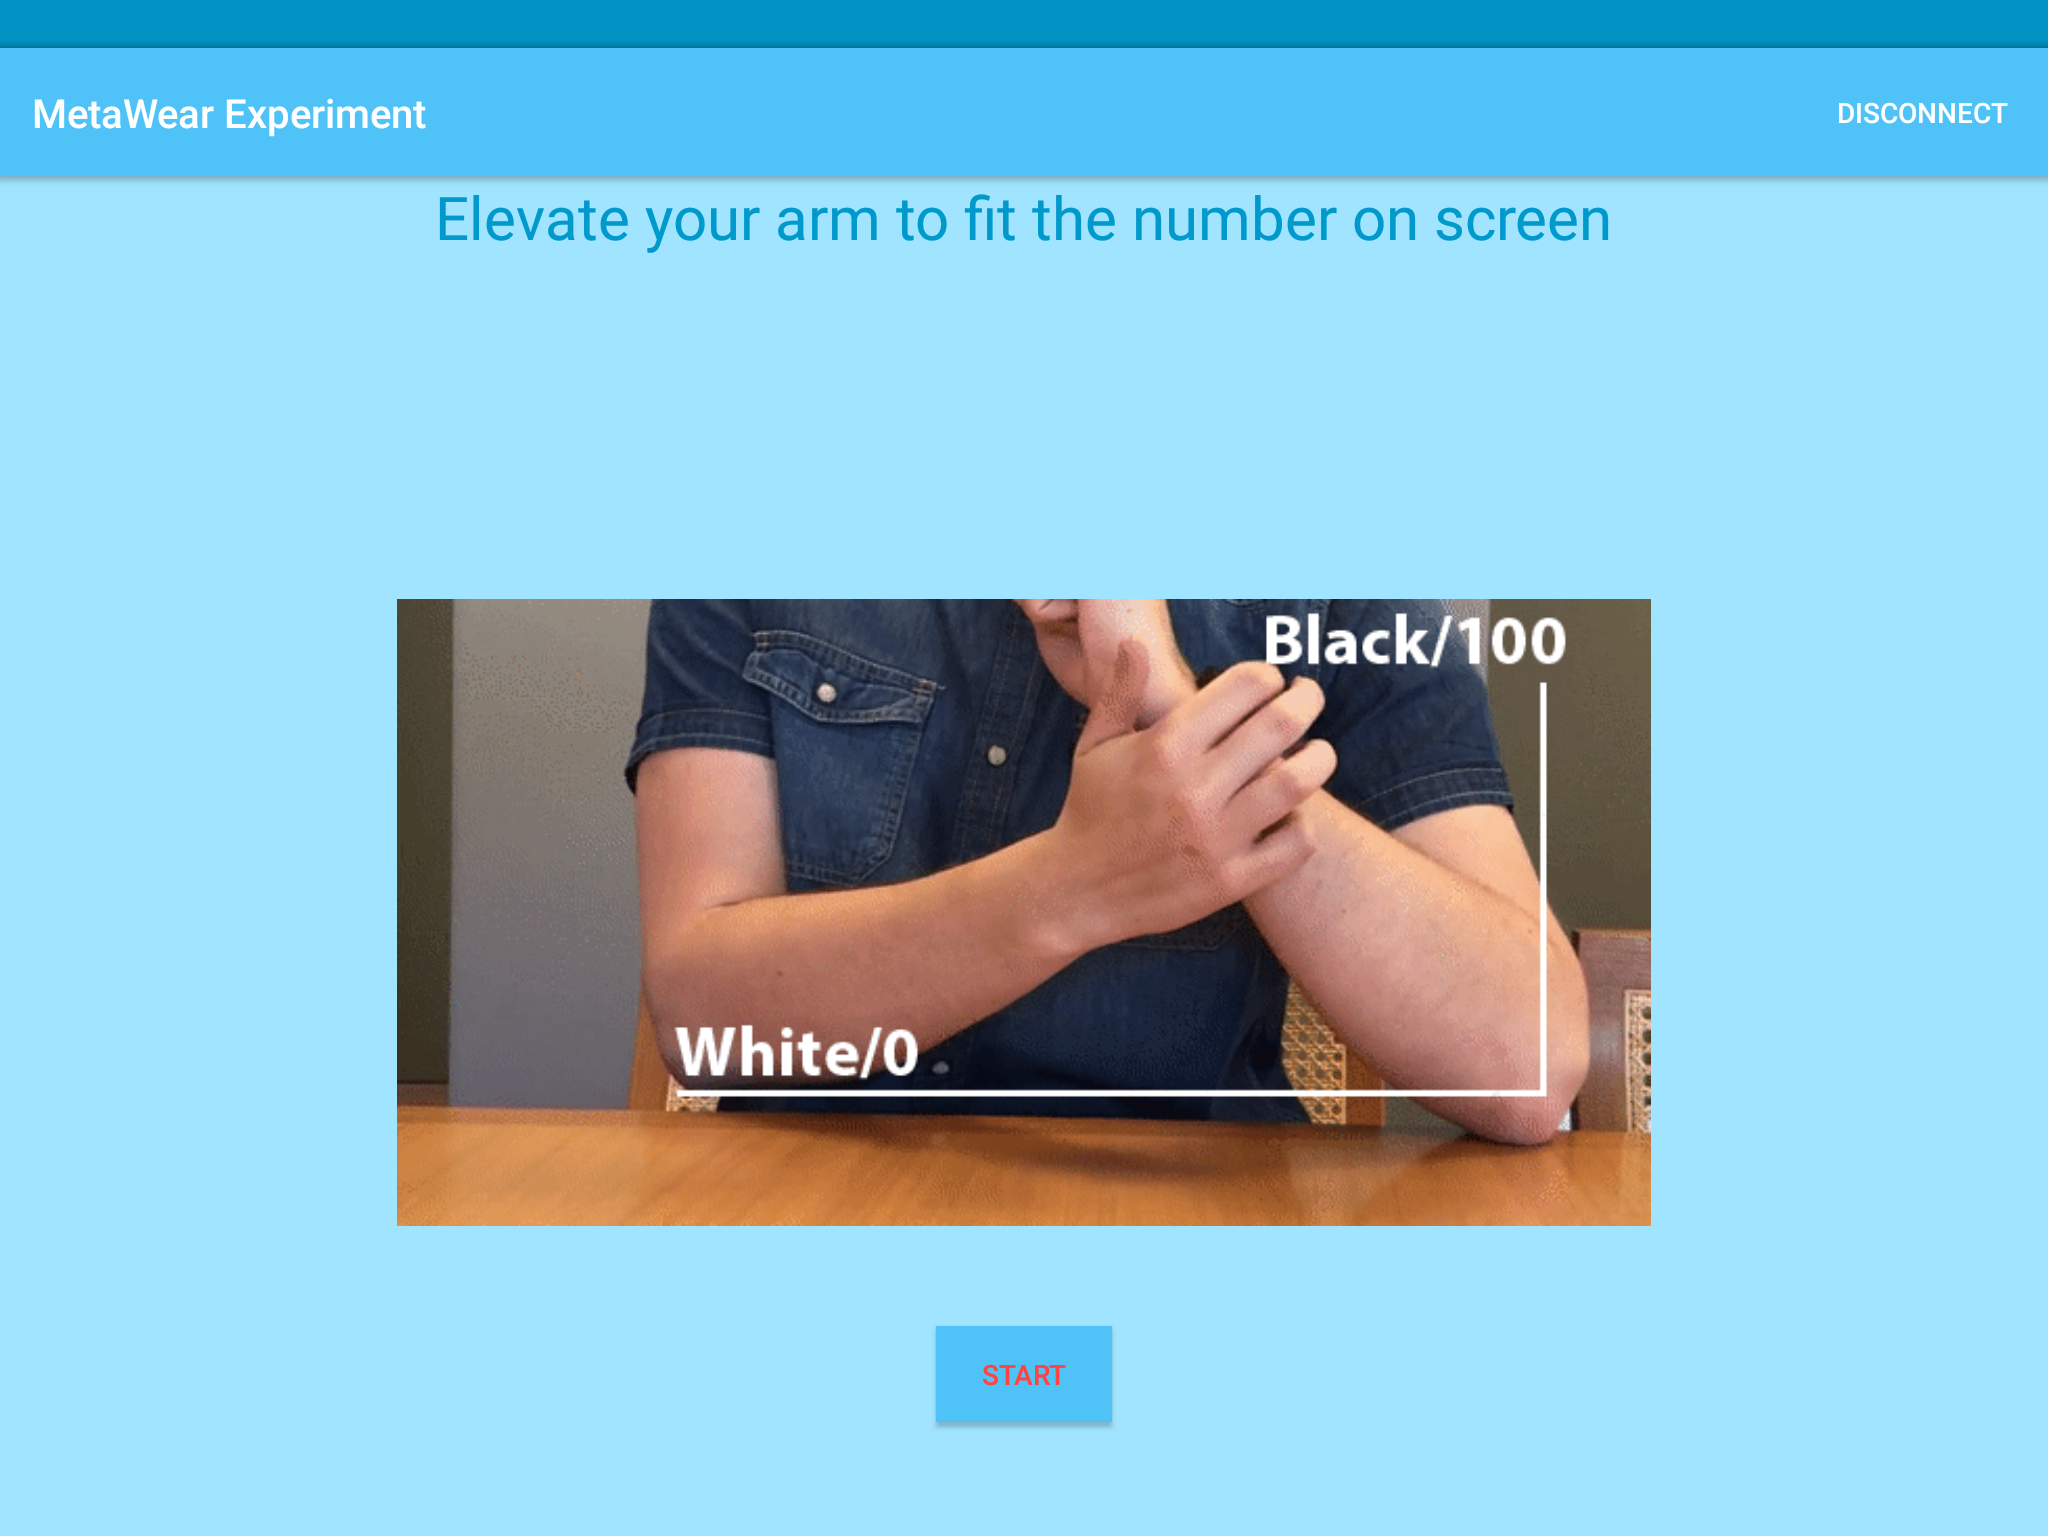
\includegraphics[width=0.95\linewidth]{figures/tablet_screen12.png}
  \captionof{figure}{arm\_num explanation screen}
  \label{app_arm_explain}
\end{minipage}%
\begin{minipage}{.55\textwidth}
  \centering
  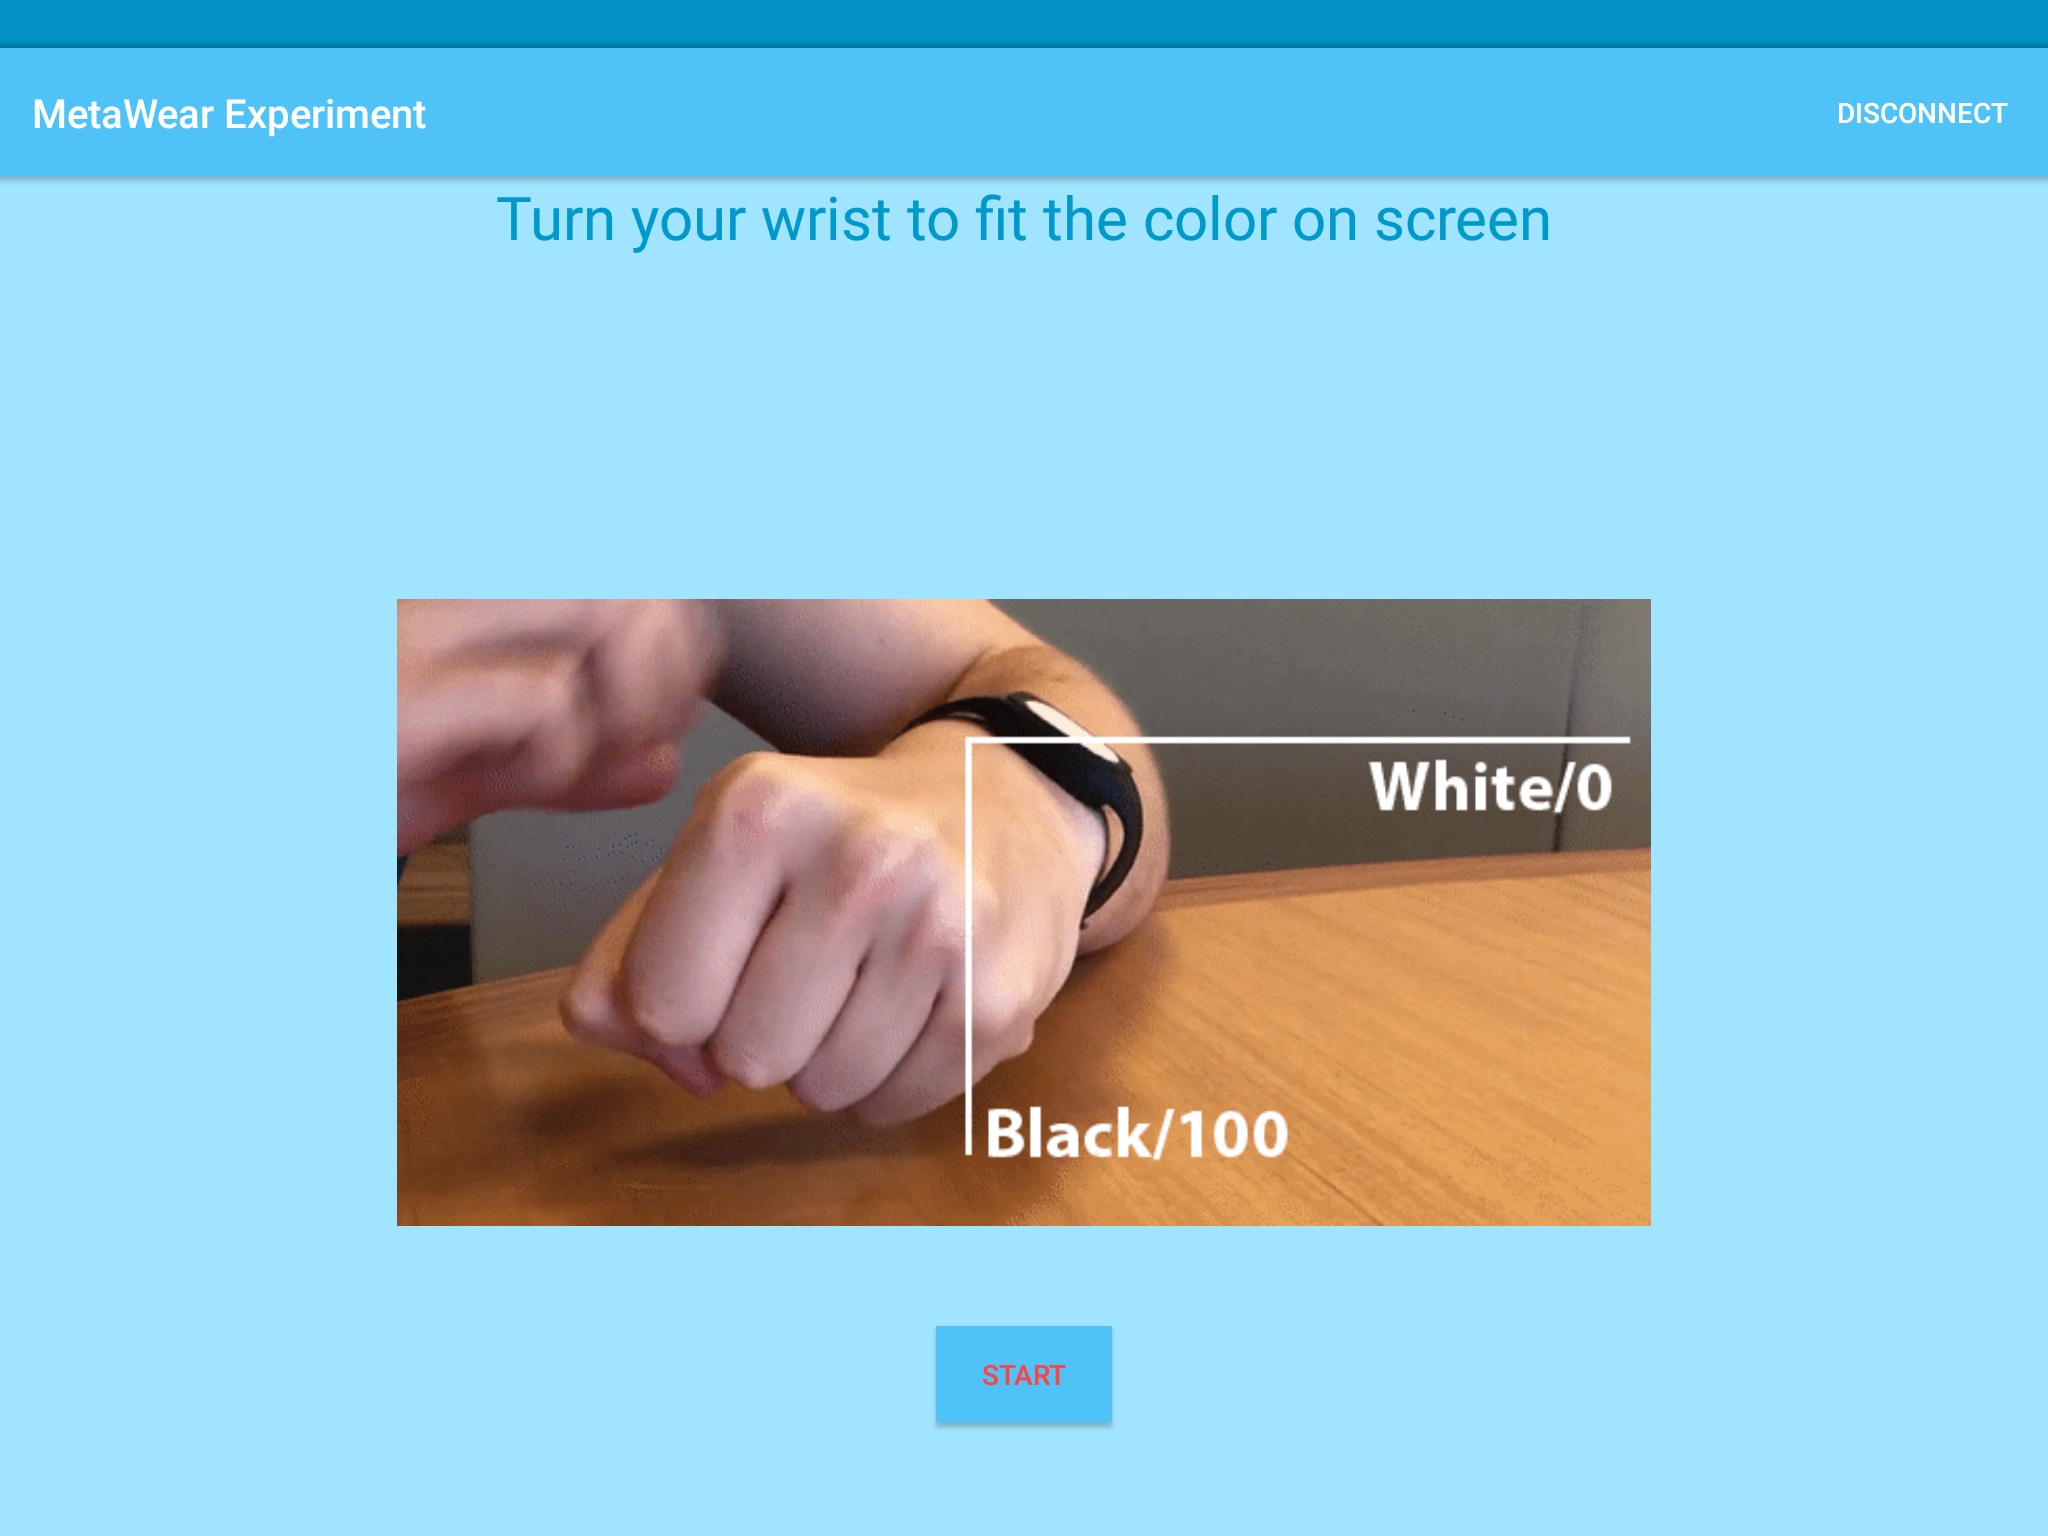
\includegraphics[width=0.95\linewidth]{figures/tablet_screen13.png}
  \captionof{figure}{wrist\_grey explanation screen}
  \label{app_wrist_explain}
\end{minipage}
\end{figure}

After the explanation screen each exercise follow the same pattern: show stimuli, wait for input, refresh input (optional), register input, next input. This pattern is repeated until the set number of stimuli has been shown and then the next exercise is started, after all six exercises are completed a \say{finish} screen is shown. The slider\_grey exercise will be used to explain this pattern in more detail. After the exercise explanation the first stimuli is shown as seen in Figure \ref{app_show_stim}, then the participant registers a input using the slider as seen in Figure \ref{app_input_slider}, a small vertical bar indicate the input. The input can be changed simply by adjusting the slider (for arm and wrist exercises the participant can just press the button on the wristband again), to register the input the participant has to press the \say{Submit} button as seen in Figure \ref{app_input_slider}. Once the input has been registered the stimuli will disappear and the participant has to press the \say{Next} button as seen in Figure \ref{app_next_stim}, this button will alternate to appear on the left and right side of the screen (this will be explained later), once the button has been pressed the next stimuli will appear (as seen in Figure \ref{app_repeat})and the process will repeat until the participant has been through the set amount of stimuli and moves on to the next exercise. In Figure \ref{app_wrist_int} we see a screen from the wrist\_num exercise where the participant has pressed the button on the wristband, beside the feedback from the wristband (light and vibration) the screen also show that the button has been pressed, but no feedback is given on what value was registered nor how well they performed. This was done on purpose to reflect the real life use case where the user wouldn't know the registered value before importing it to the companion app. In Figure \ref{app_finish} we see the \say{Finish} screen after the participant has completed the experiment. All app screens shown here plus a couple extra can be seen in larger scale in Appendix \ref{ex_app_screens}.

\begin{figure}[h!]
\centering
\begin{minipage}{.55\textwidth}
  \centering
  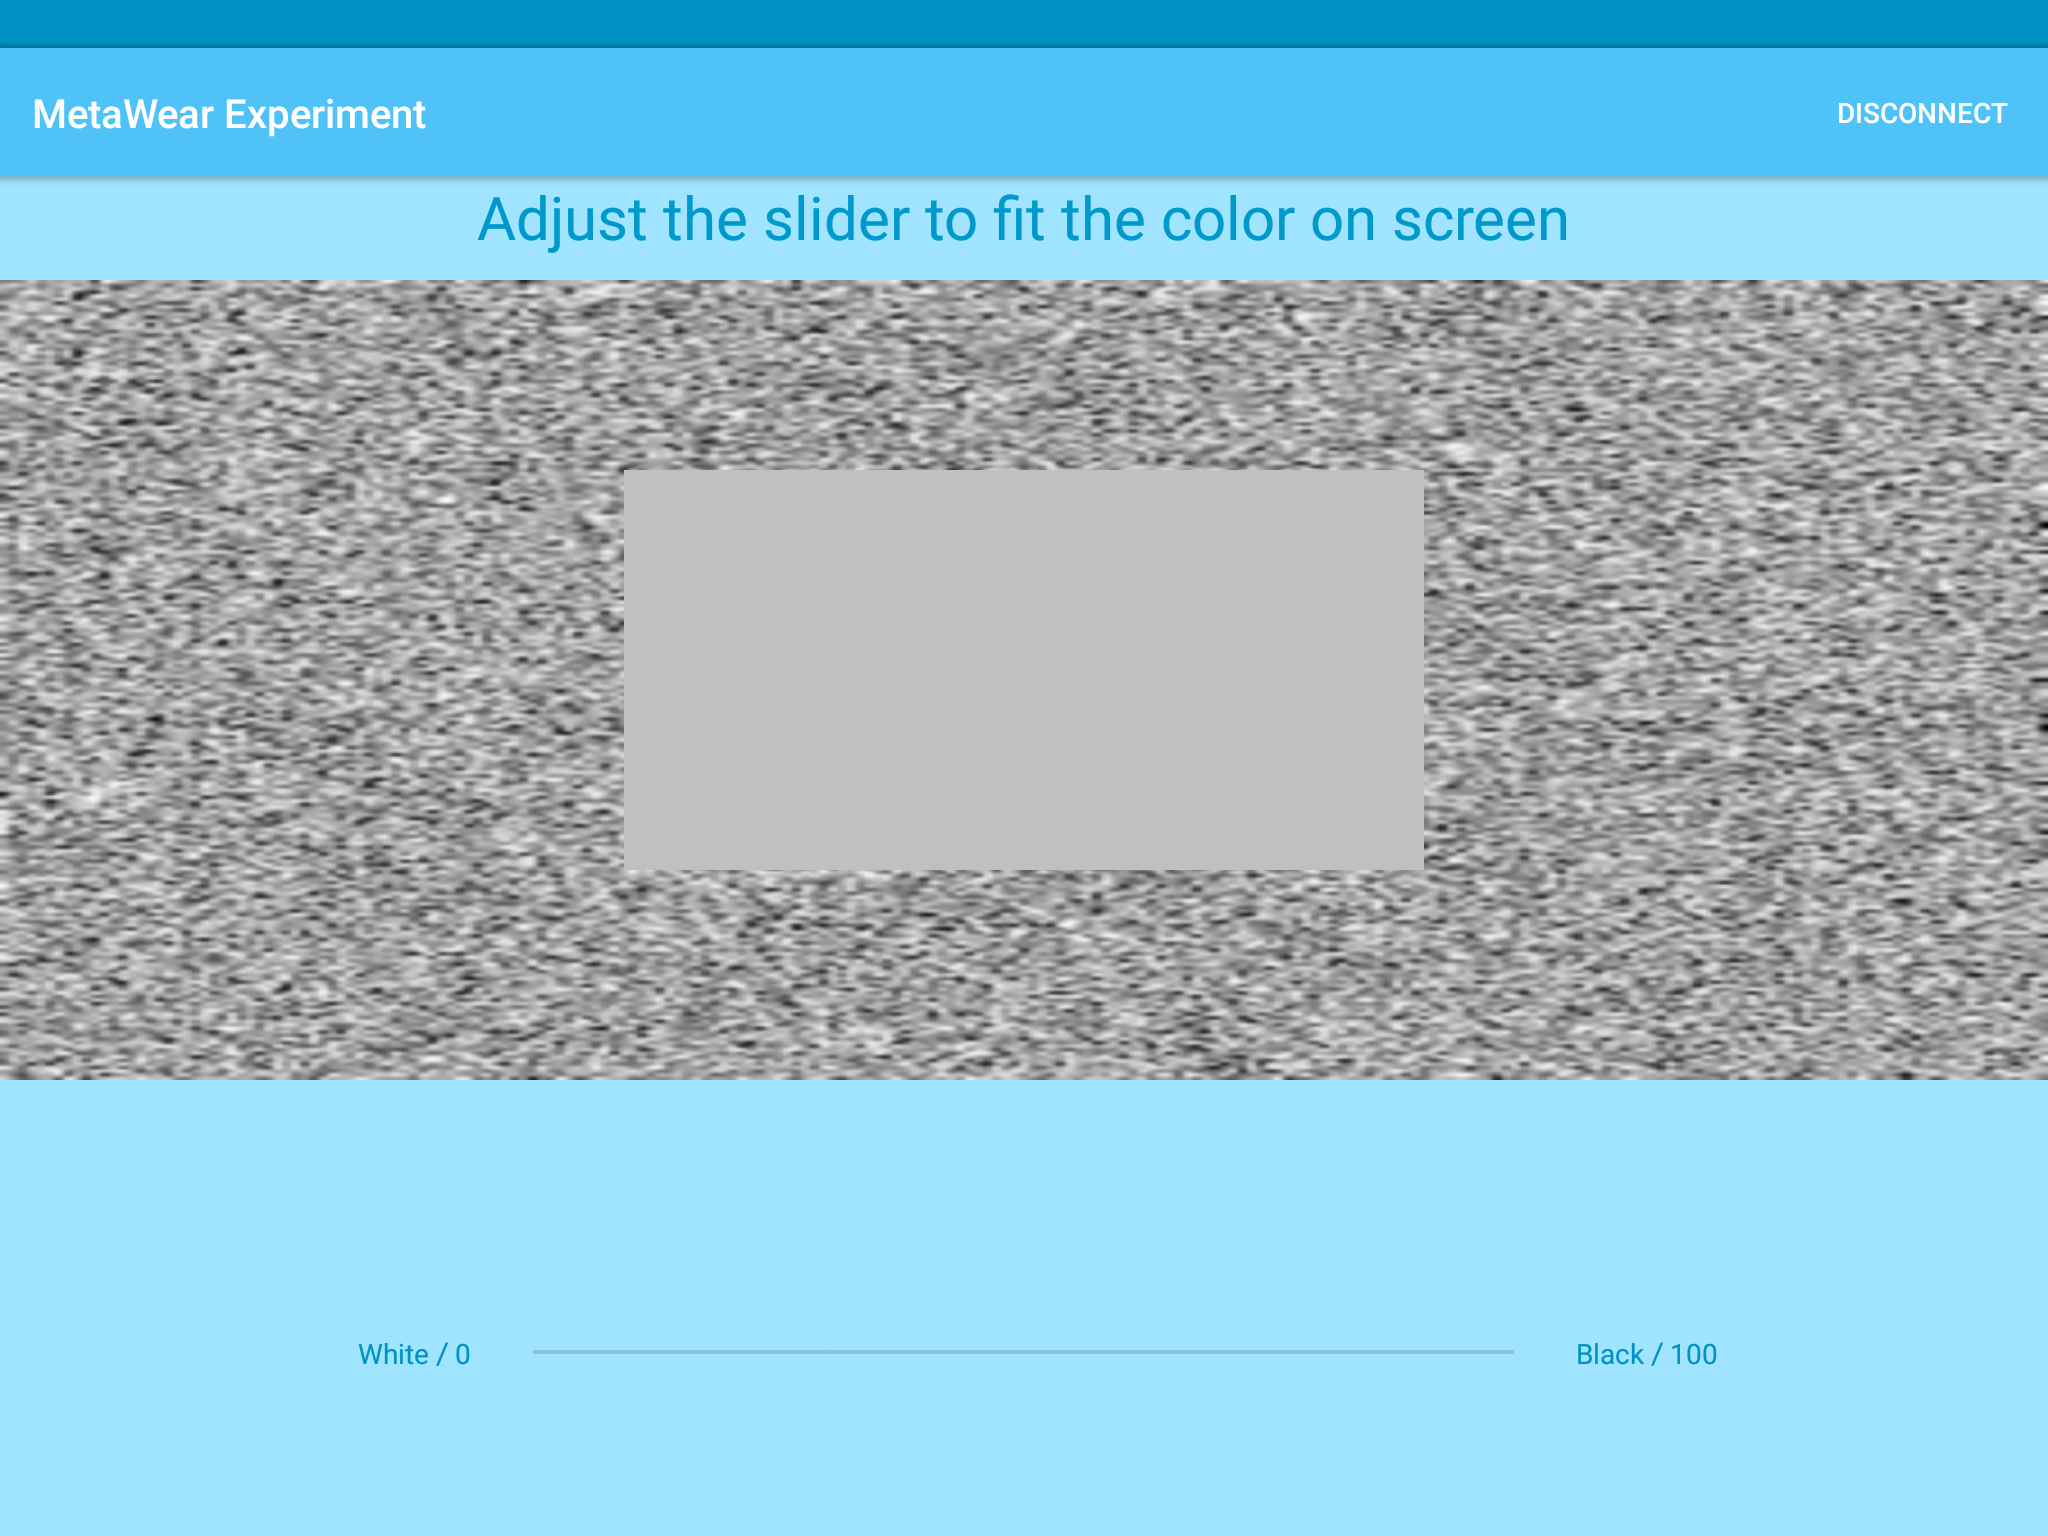
\includegraphics[width=0.95\linewidth]{figures/tablet_screen7.png}
  \captionof{figure}{Show stimuli screen with shade of grey}
  \label{app_show_stim}
\end{minipage}%
\begin{minipage}{.55\textwidth}
  \centering
  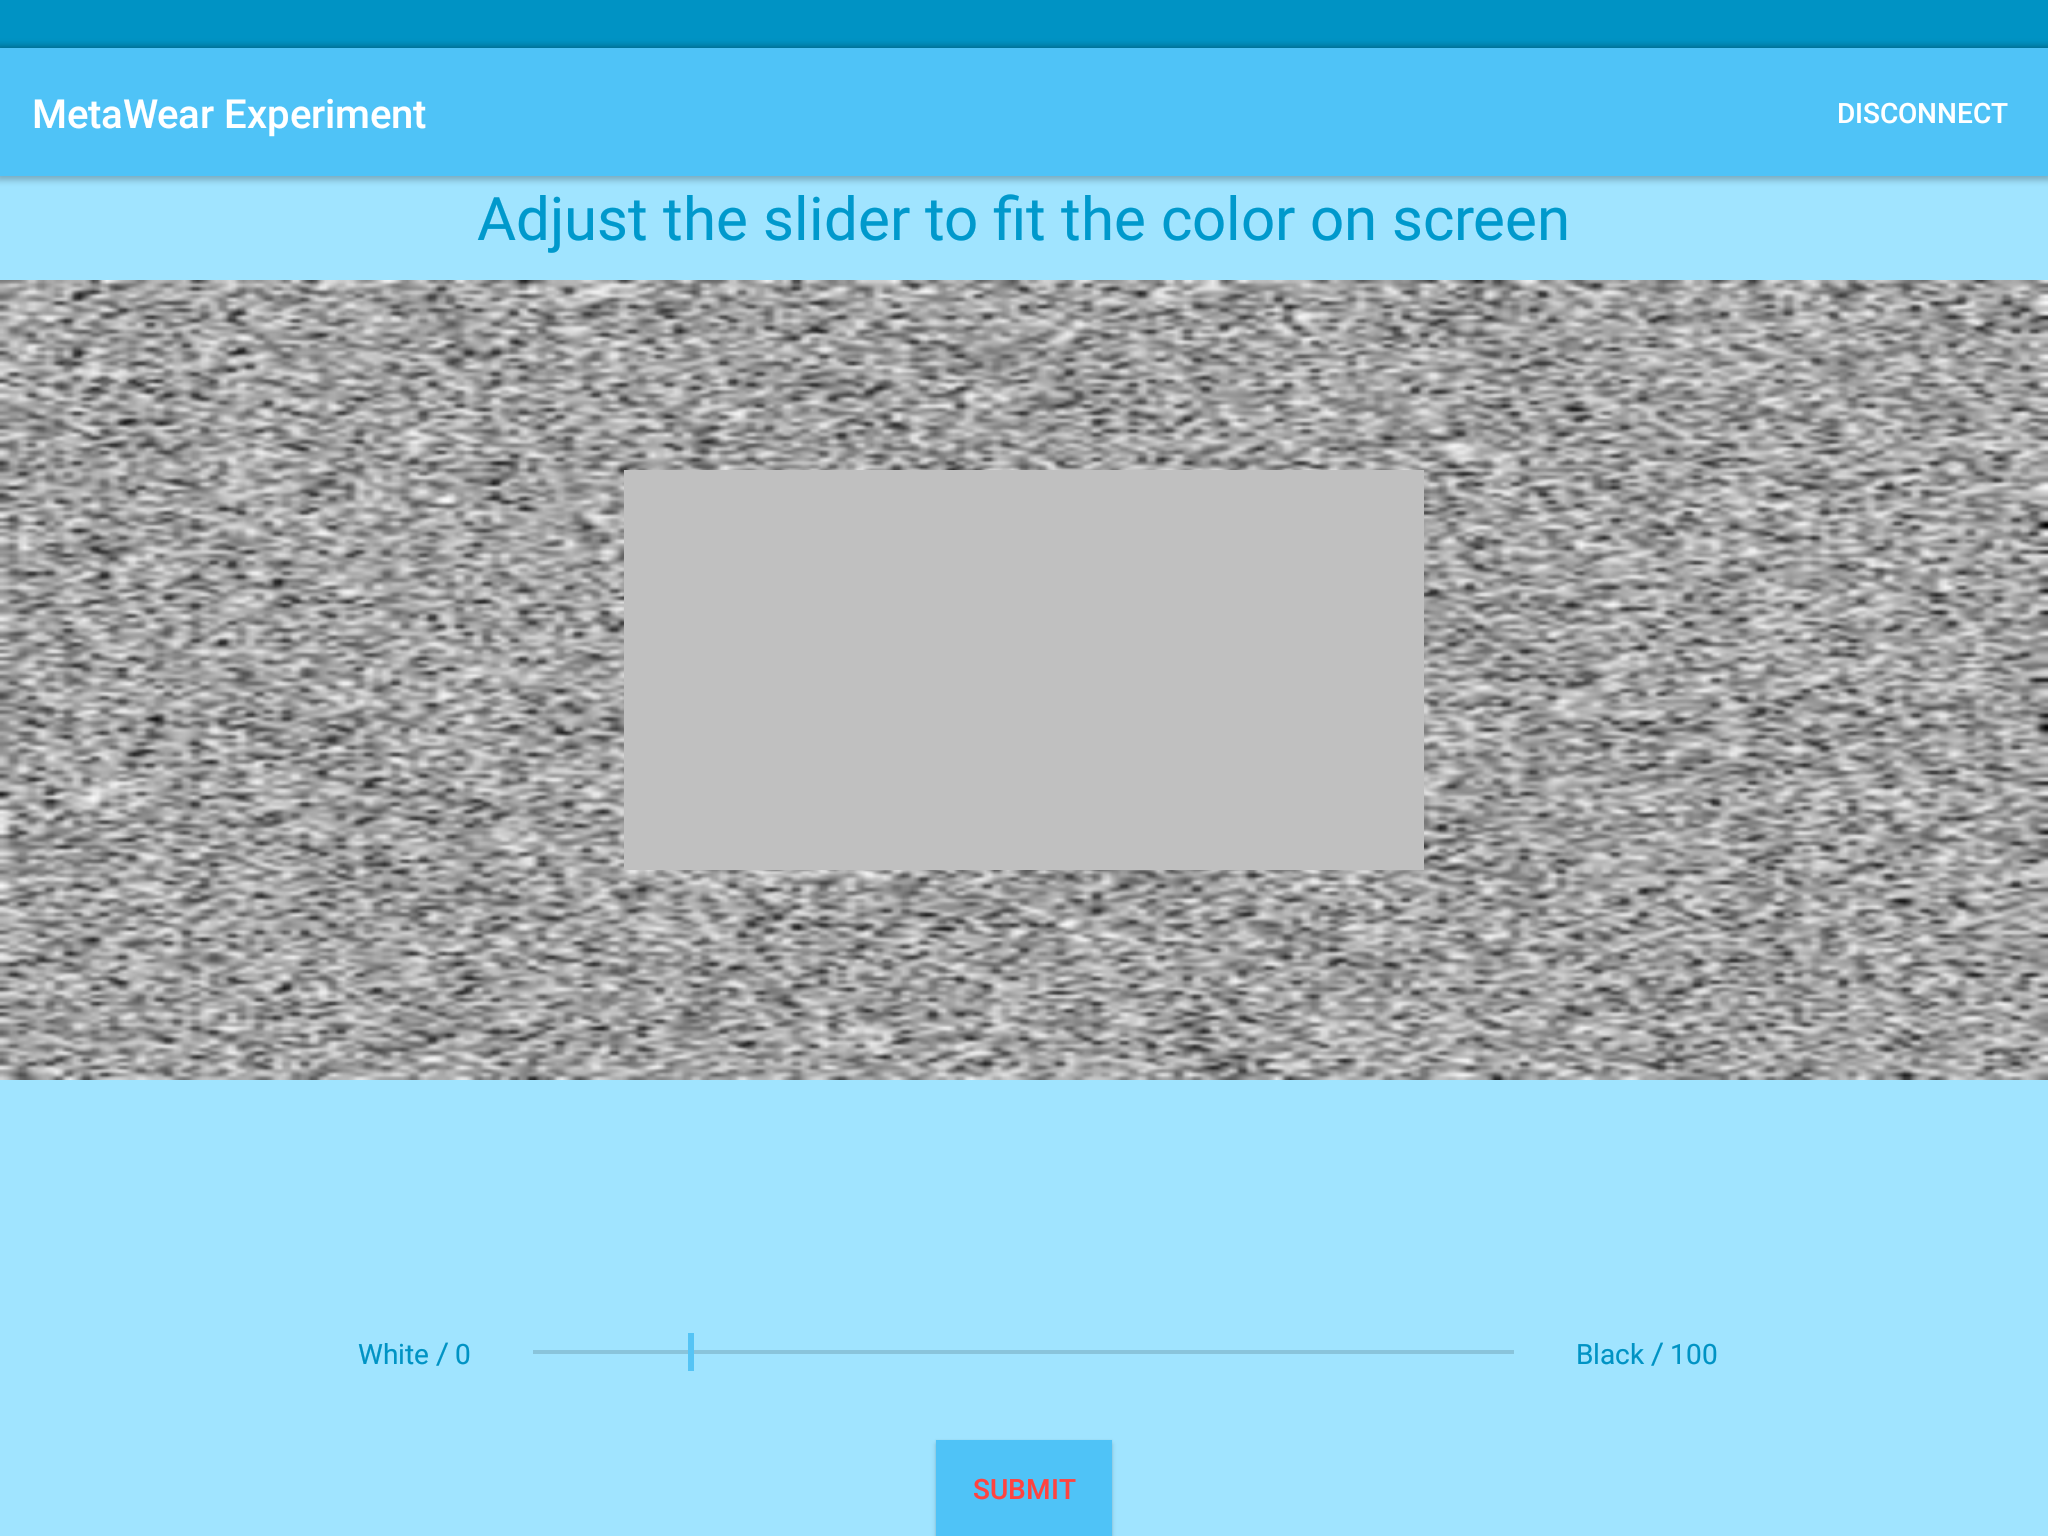
\includegraphics[width=0.95\linewidth]{figures/tablet_screen8.png}
  \captionof{figure}{Participant has given an input using the slider}
  \label{app_input_slider}
\end{minipage}
\end{figure}

\begin{figure}[h!]
\centering
\begin{minipage}{.55\textwidth}
  \centering
  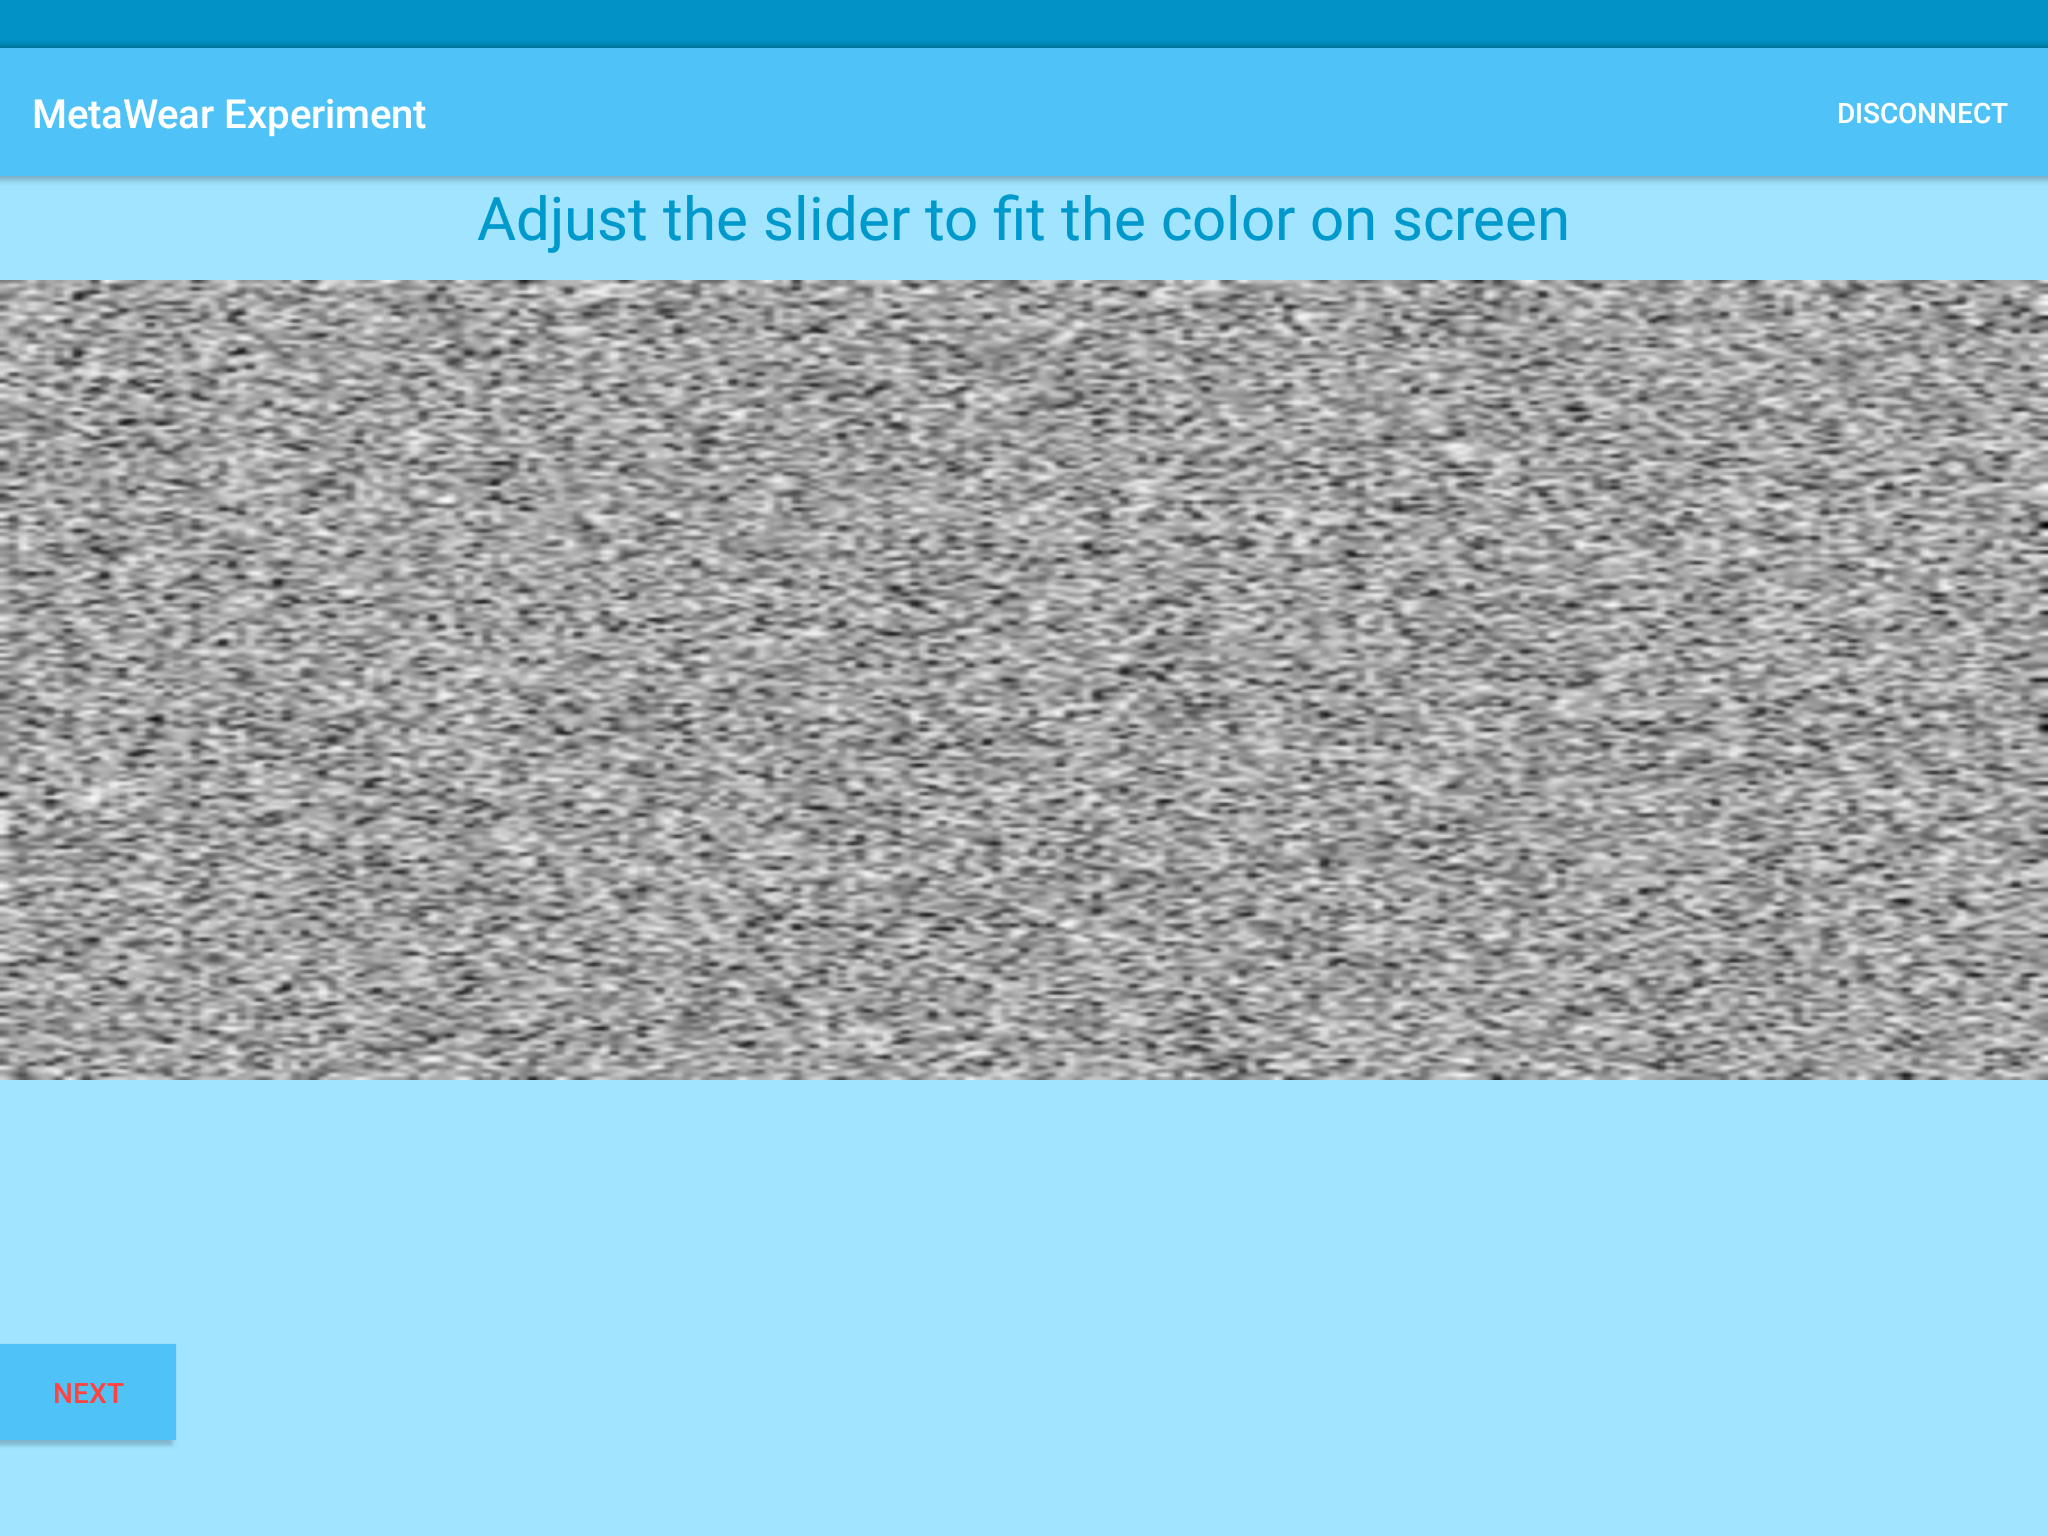
\includegraphics[width=0.95\linewidth]{figures/tablet_screen9.png}
  \captionof{figure}{Next stimuli screen}
  \label{app_next_stim}
\end{minipage}%
\begin{minipage}{.55\textwidth}
  \centering
  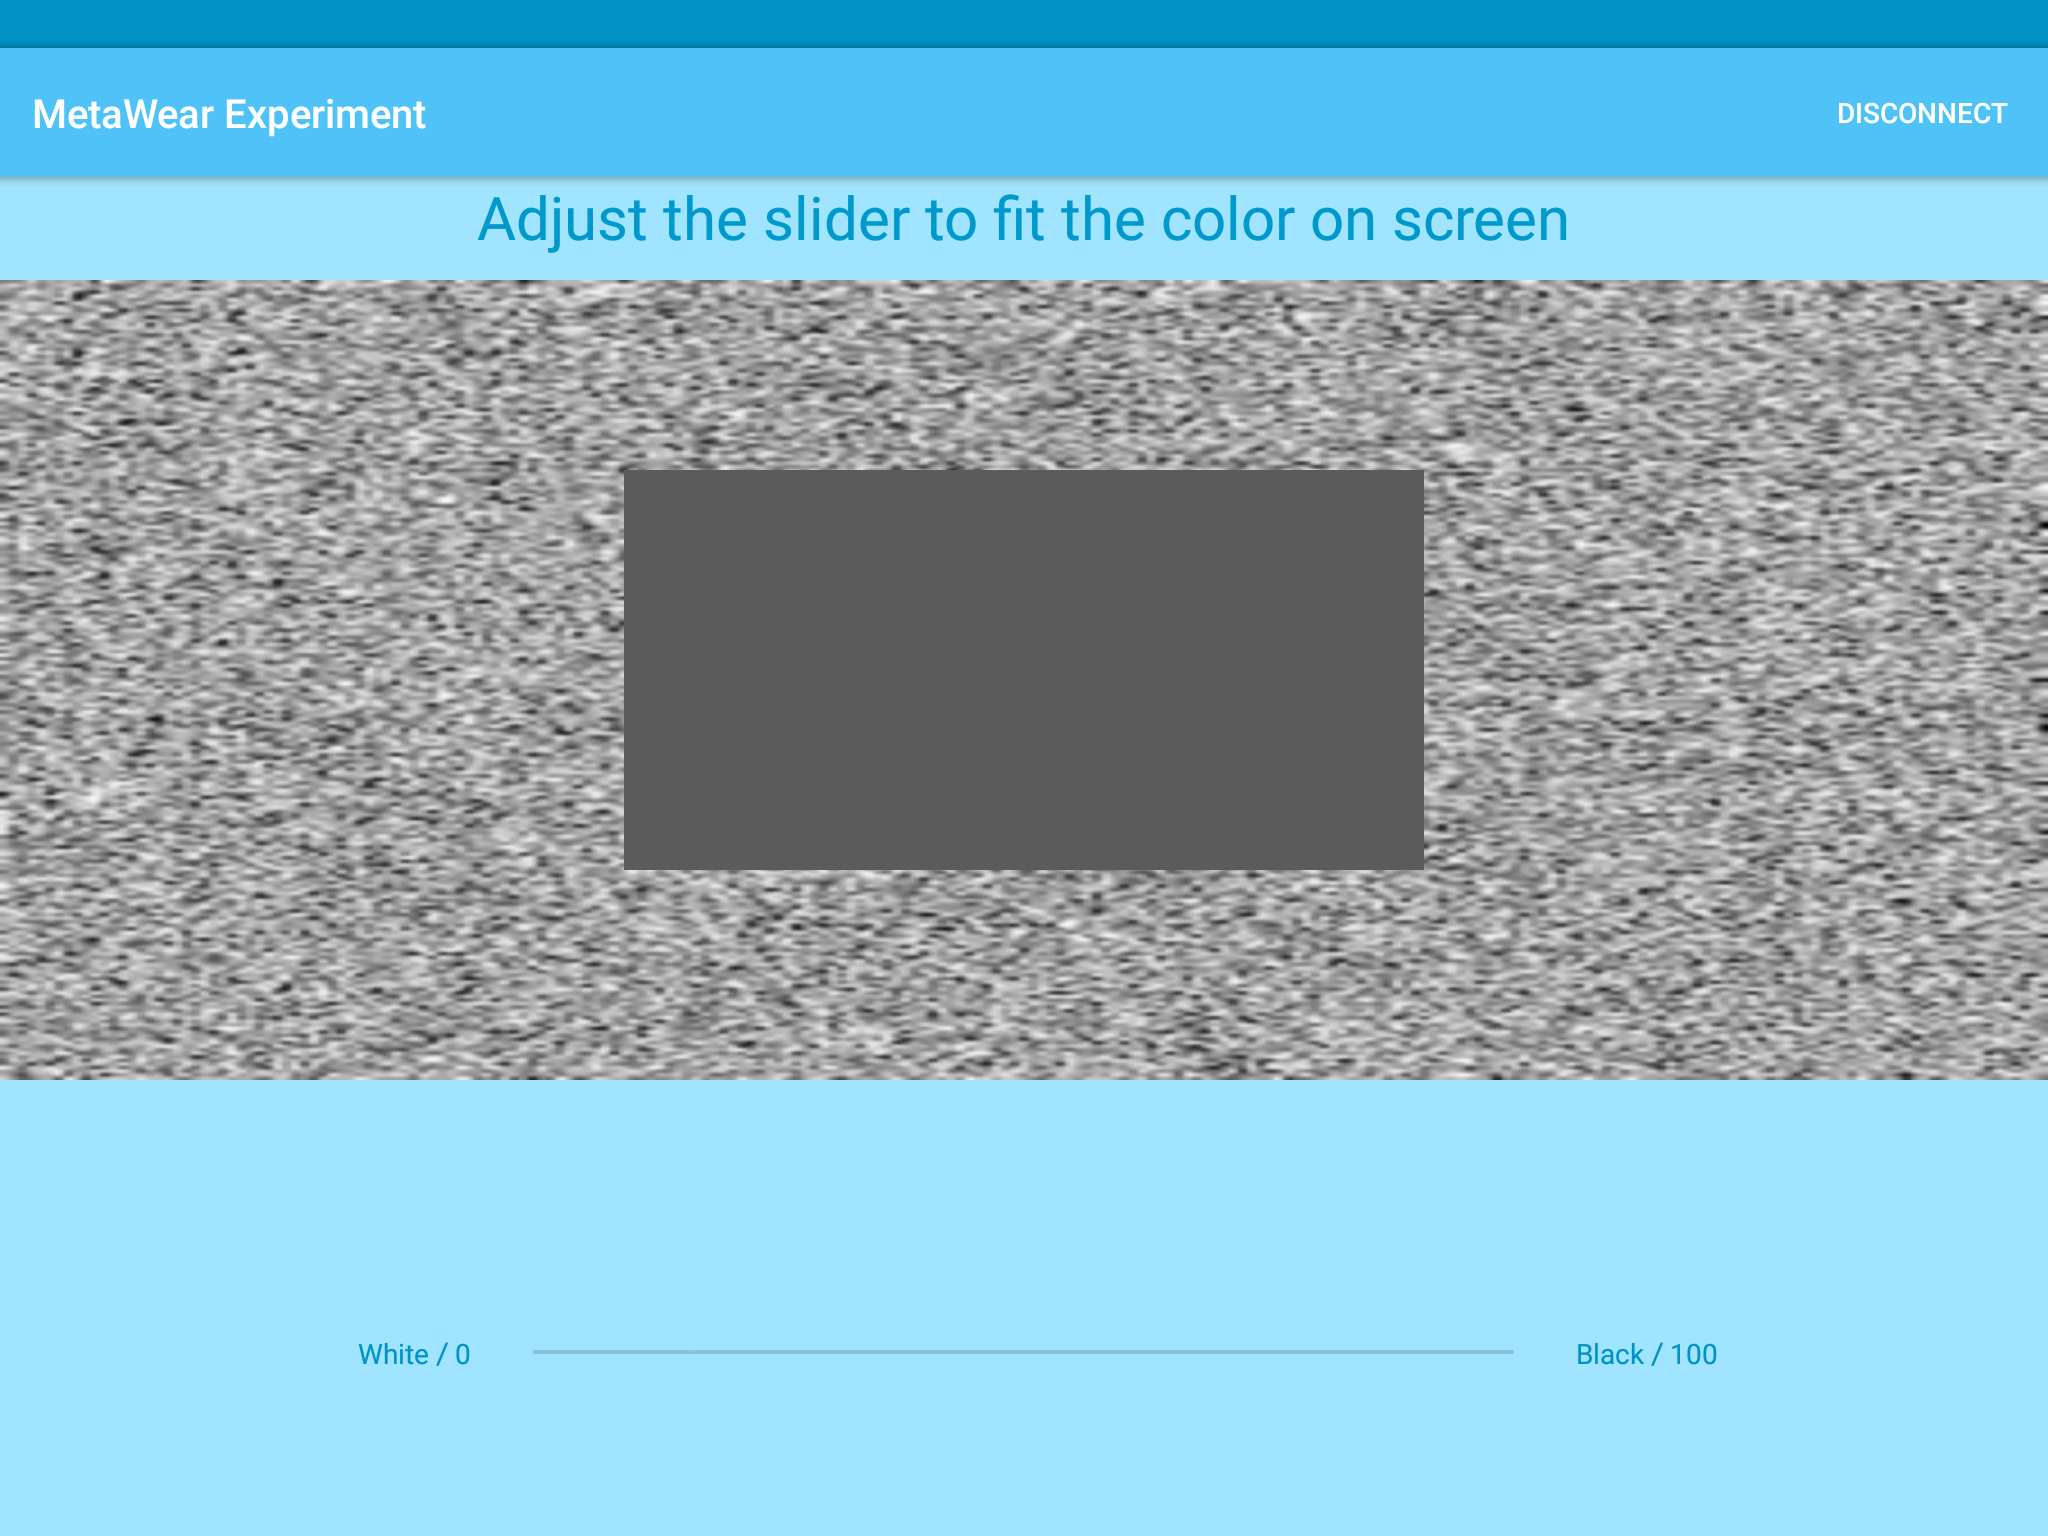
\includegraphics[width=0.95\linewidth]{figures/tablet_screen10.png}
  \captionof{figure}{Pattern is repeated}
  \label{app_repeat}
\end{minipage}
\end{figure}

\begin{figure}[h!]
\centering
\begin{minipage}{.55\textwidth}
  \centering
  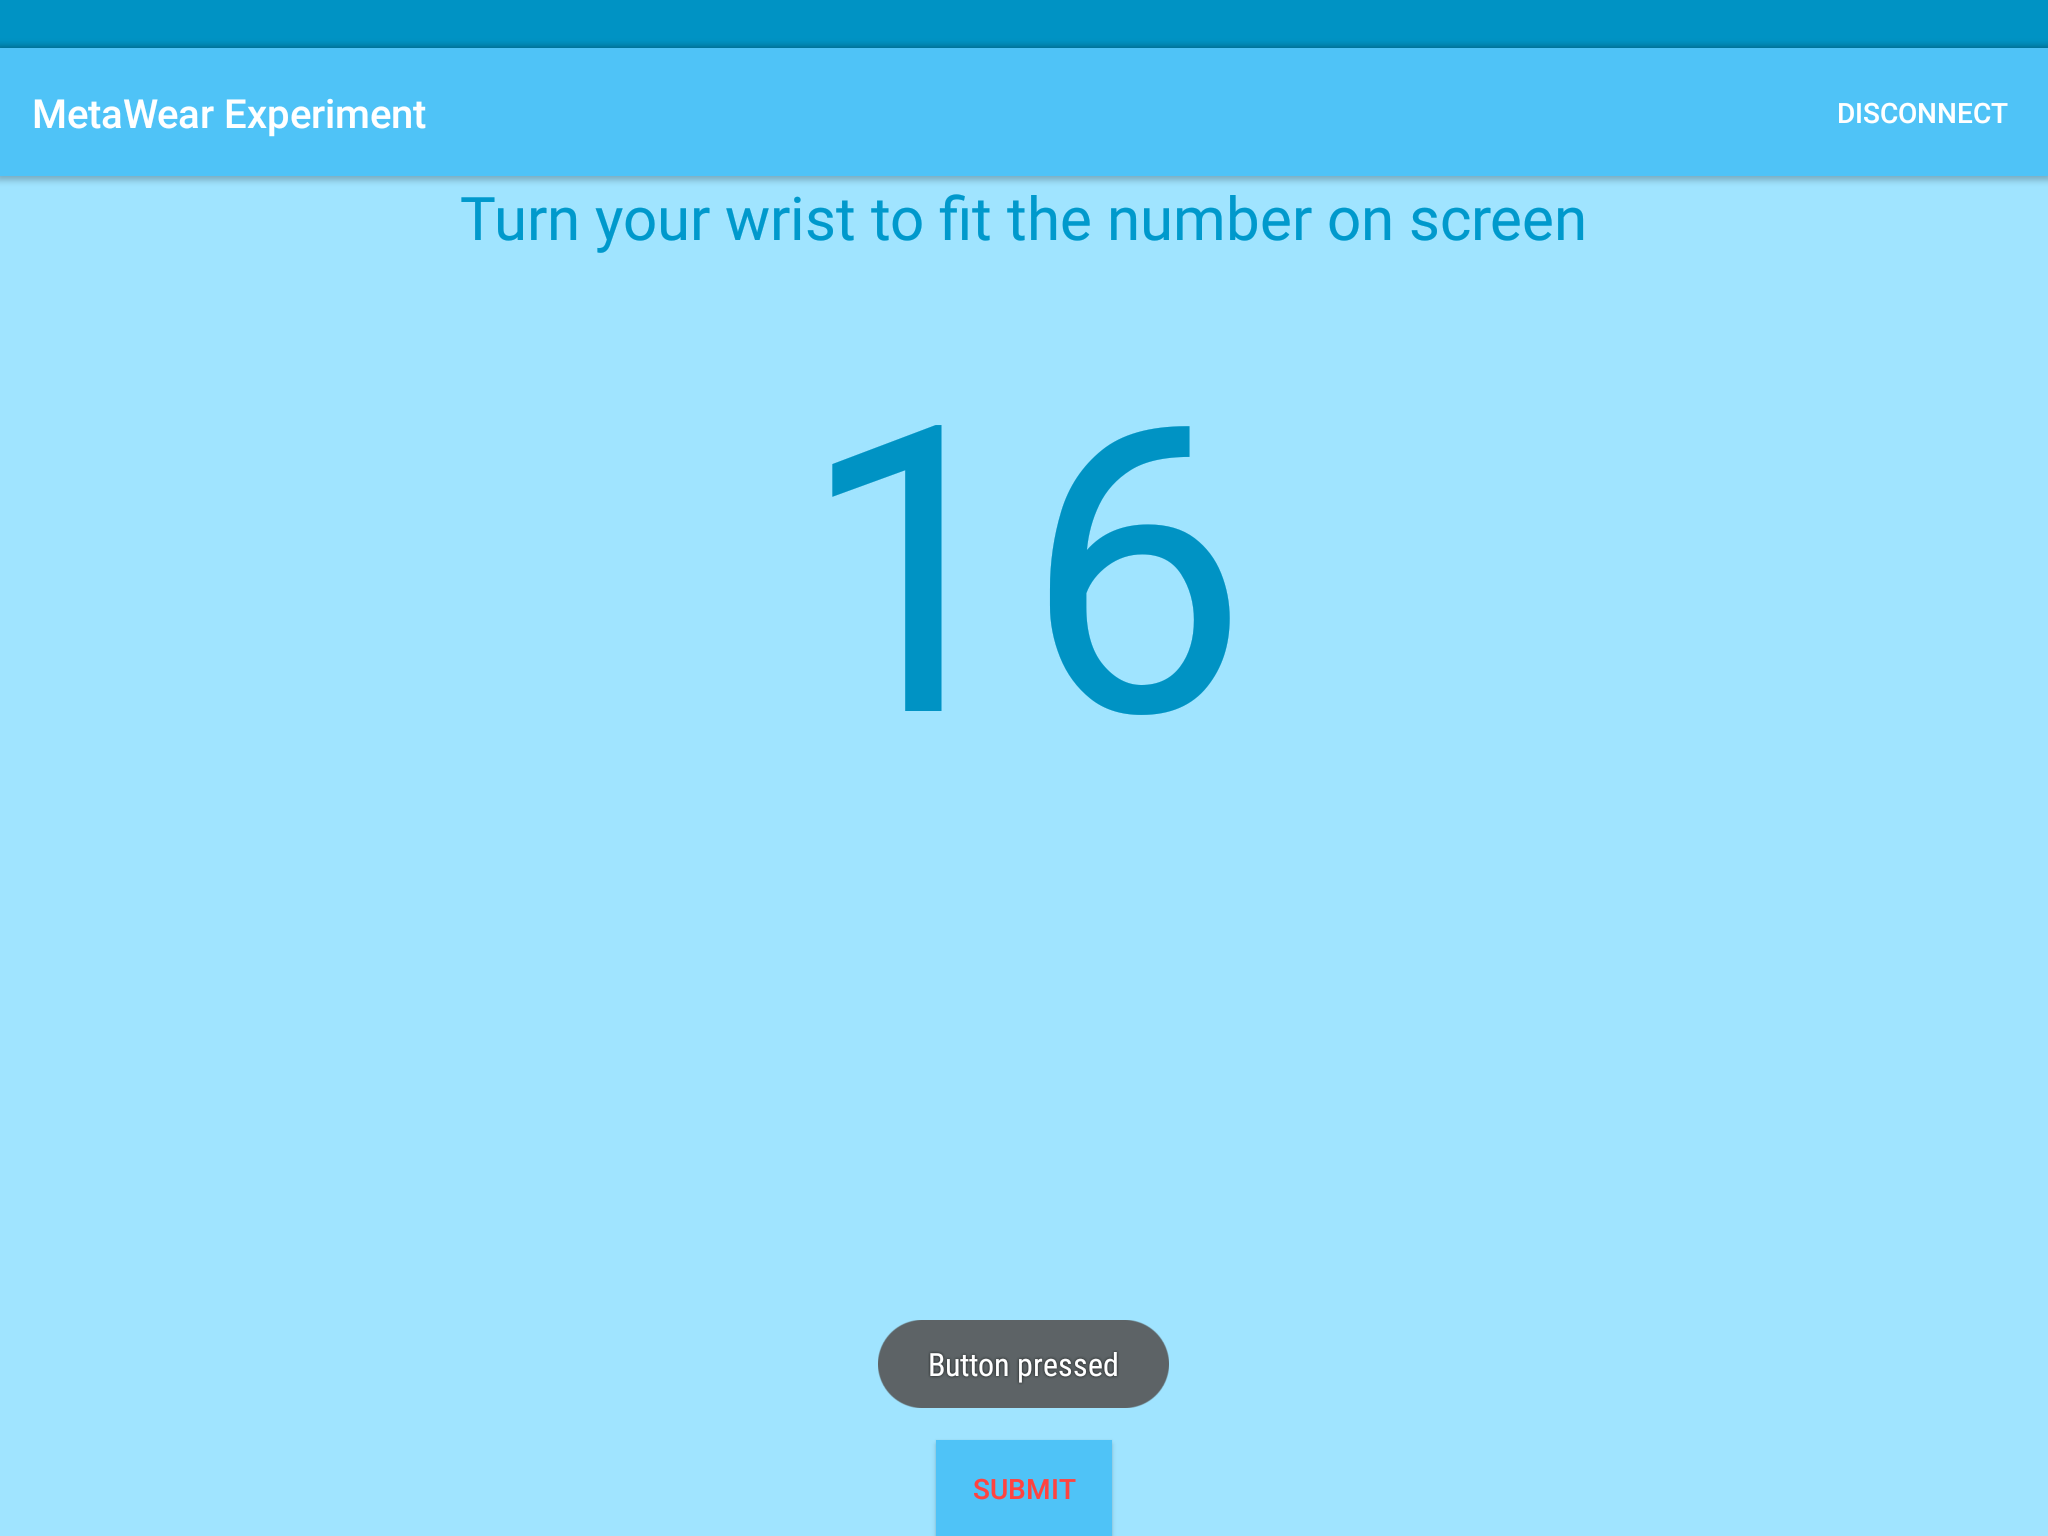
\includegraphics[width=0.95\linewidth]{figures/tablet_screen16.png}
  \captionof{figure}{Input registered from wristband with integer stimuli}
  \label{app_wrist_int}
\end{minipage}%
\begin{minipage}{.55\textwidth}
  \centering
  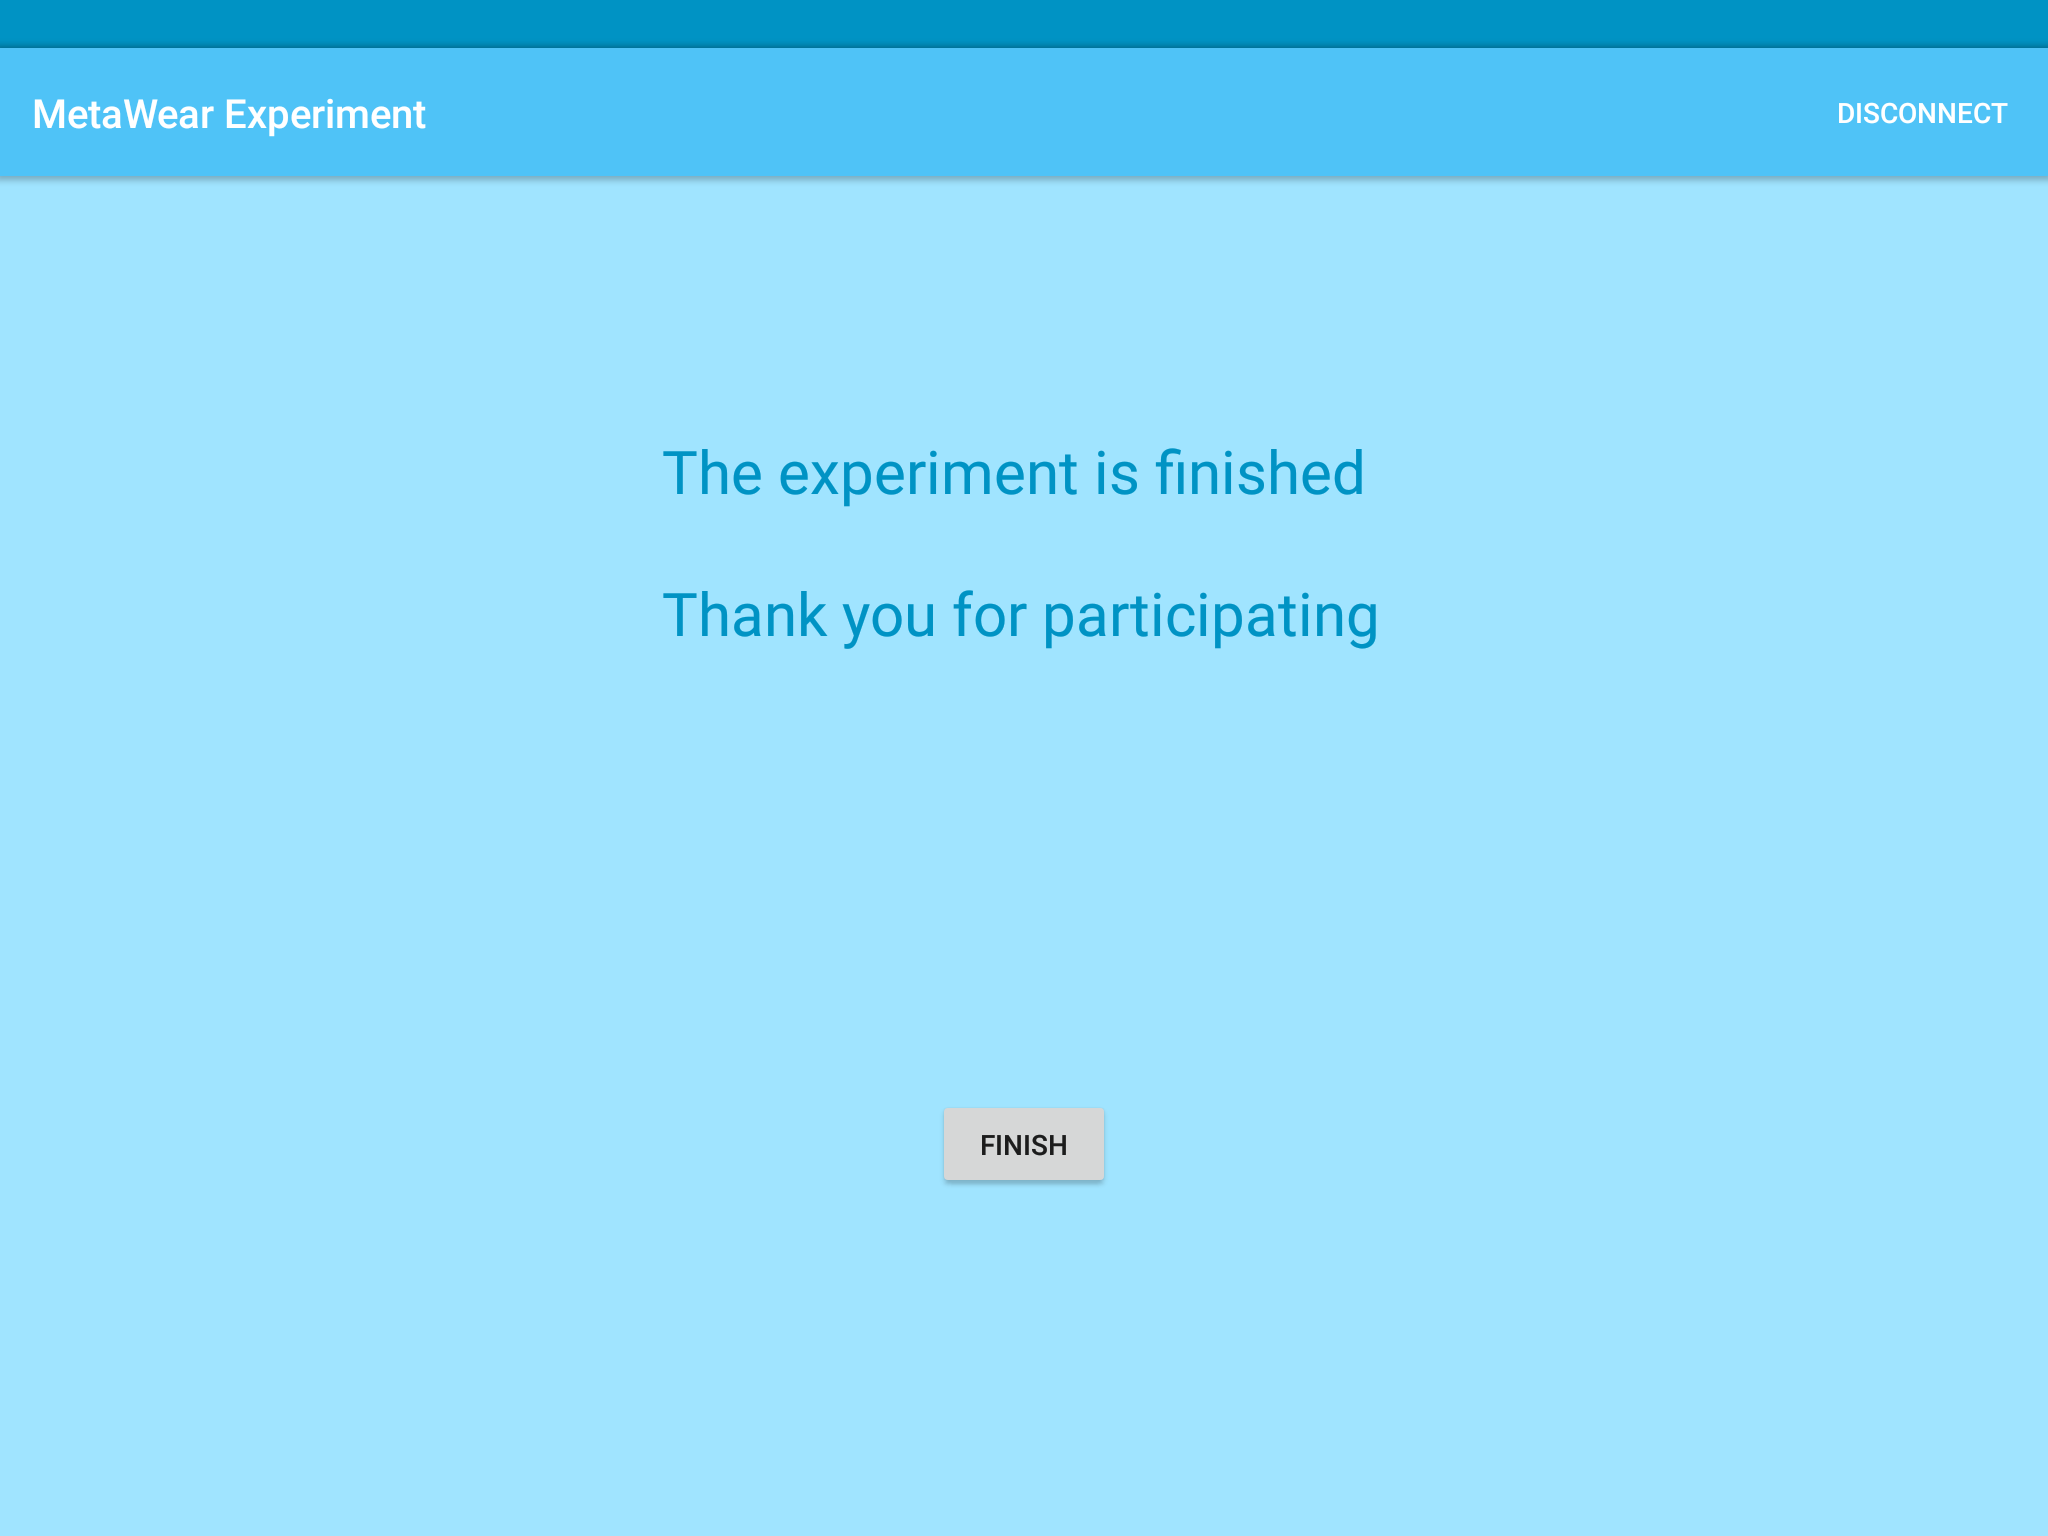
\includegraphics[width=0.95\linewidth]{figures/tablet_screen17.png}
  \captionof{figure}{Finished experiment screen}
  \label{app_finish}
\end{minipage}
\end{figure}

The stimuli for each exercise follow a specific set of rules. First of all the stimuli for each exercise is independent. For num exercises the stimuli is generated by creating an array of integers from 0-100, e.g. [0, 1, 2 .. 98, 99, 100]. This array is shuffled so the order is random. When a stimuli is needed the first element in the array is used, once used it is removed from the array. Once the array is empty the process is repeated. For grey exercises the process is the same, but the array consist of integers from 0-49, here 0 correspond to pure white, 49 is pure black and the rest are the shaded of grey in between. The shaded of grey are the same as used by Matejka et al.\cite{grey} as seen in Figure \ref{50shades}, where each shade is of equal distance from each other in the CIELAB color space\cite{cielab}. What this means is that the order of stimuli is completely random, but the distribution of stimuli is completely even, this means that for each participant the stimuli is random but not repeated, while keeping the overall even distribution between participants. Again emphasizing on the fact that the stimuli for each exercise is independent.

The data collected from the experiment is described in Table \ref{data_in}. Data is recorded whenever the participant pressed the submit button for each trial. With the six exercises each having 20 trials, this results in 120 data points for each participant and a total of 2880 data points for the complete experiment. Most of the data is self explanatory and doesn't need further explanation than the table. The \say{type} refers to the exercise. \say{type\_order} refers to the order of the exercises, this data is redundant since it can be deducted based on the \say{id} and Table \ref{latin}. \say{stim\_order} is the order the stimuli had and is also redundant since it can be deducted based on the time stamp, but if any of these were to be investigated this would greatly reduce the work. The \say{pitch}, \say{roll} and \say{yaw} are the Euler angles recorded, these could be used to change the mapping functions from Euler angles to scaled value without needing to redo experiment (these values are only recorded for wrist and arm exercises). The \say{reaction\_time} is recorded from when the stimuli was shown on screen until the participant pressed the submit button. The data collected is saved to a CSV file in the apps internal storage, and can be exported from the settings screen as described earlier. Beside this data, a separate data file was created where to total time taken to complete the experiment (from pressing start in Figugre \ref{app_ex_start} to the finsih screen was shown).


% Please add the following required packages to your document preamble:
% \usepackage{graphicx}
\begin{table}[h!]
\centering
\resizebox{\textwidth}{!}{%
\begin{tabular}{lll}
column name                          & type                                  & descriptiom                                                                                                                                                            \\ \hline
\multicolumn{1}{|l|}{id}             & \multicolumn{1}{l|}{int}              & \multicolumn{1}{l|}{Uniqe id for each particpant}                                                                                                                      \\ \hline
\multicolumn{1}{|l|}{gender}         & \multicolumn{1}{l|}{String}           & \multicolumn{1}{l|}{Participant gender: "Male" or "Female"**}                                                                                                          \\ \hline
\multicolumn{1}{|l|}{age}            & \multicolumn{1}{l|}{int}              & \multicolumn{1}{l|}{Participant age**}                                                                                                                                 \\ \hline
\multicolumn{1}{|l|}{time}           & \multicolumn{1}{l|}{Date object}      & \multicolumn{1}{l|}{Timestamp when input was registered}                                                                                                               \\ \hline
\multicolumn{1}{|l|}{type}           & \multicolumn{1}{l|}{String}           & \multicolumn{1}{l|}{\begin{tabular}[c]{@{}l@{}}Type of exercise: "slider\_grey", "slider\_num", "wrist\_grey",\\ "wrist\_num", "arm\_grey" or "arm\_num"\end{tabular}} \\ \hline
\multicolumn{1}{|l|}{type\_order}    & \multicolumn{1}{l|}{int}              & \multicolumn{1}{l|}{Order for the type of exercise: 0-5*}                                                                                                              \\ \hline
\multicolumn{1}{|l|}{stim\_order}    & \multicolumn{1}{l|}{int}              & \multicolumn{1}{l|}{Order for the stimuli: 0-49 or 0-100*}                                                                                                             \\ \hline
\multicolumn{1}{|l|}{stim}           & \multicolumn{1}{l|}{int}              & \multicolumn{1}{l|}{Stimuli: 0-49 or 0-100}                                                                                                                            \\ \hline
\multicolumn{1}{|l|}{response}       & \multicolumn{1}{l|}{double}           & \multicolumn{1}{l|}{Response: 0.0-49.0 or 0.0-100.0}                                                                                                                   \\ \hline
\multicolumn{1}{|l|}{pitch}          & \multicolumn{1}{l|}{double or String} & \multicolumn{1}{l|}{Value of pitch for exercises using the wristband, else "NA"**}                                                                                     \\ \hline
\multicolumn{1}{|l|}{roll}           & \multicolumn{1}{l|}{double or String} & \multicolumn{1}{l|}{Value of roll for exercises using the wristband, else "NA"**}                                                                                      \\ \hline
\multicolumn{1}{|l|}{yaw}            & \multicolumn{1}{l|}{double or String} & \multicolumn{1}{l|}{Value of yaw for exercises using the wristband, else "NA"**}                                                                                       \\ \hline
\multicolumn{1}{|l|}{reaction\_time} & \multicolumn{1}{l|}{long}             & \multicolumn{1}{l|}{\begin{tabular}[c]{@{}l@{}}Time in milliseconds from the stimuli was shown\\ until a response was registred\end{tabular}}                          \\ \hline
                                     &                                       & *Redundant data. **Data not investigated                                                                                                                              
\end{tabular}%
}
\caption{Structure of Collected Data}
\label{data_in}
\end{table}

\subsection{Other}
Beside the described hardware and software a small foam pad was used for the participant to place their elbow on, this reduced fatigue. A power bank was connected to the tablet to keep the it from running out of power and to keep the angle between the display and table at 15º, this reducing the glance in the display from the ceiling lights and gave a better viewing angle. 



% % % % % % % % % % % % % % % % % % % 
% PROCEDURE % PROCEDURE % PROCEDURE %
% % % % % % % % % % % % % % % % % % %
\section{Procedure}
Each participant completed the experiment in one continuous sitting, the whole process took approximately 15 minutes from the entered the room until they left. First participant was seated in front of the tablet and assisted to wear the wristband correctly. They were told to wear it on the arm the felt most comfortable with, but all participants choose their left arm. Then the participants was informed of how the device worked, they where shown the same gestures described in Figure \ref{pitch} and \ref{roll} (the gestured was performed on them, they weren't shown the Figures). It was made clear that the horizontal position would register as a minimum value, that the horizontal position would register a maximal value. They were instructed about how the scaled value would decrease if they performed the gesture beyond the vertical point.

They were then taken to the \say{Train} screen of the app, where they were given 1-2 minutes with each gesture to get a sense of the scale. They were asked to produce an input as close to zero and ten as possible. Again they were told about the what would happen if the went beyond the gesture, and they could see the result. They where then instructed to after each input with the wristband to lay their hand flat on the table. This was to have the same baseline for each input.

After training they were instructed on the structure of the experiment. They were told about the three input methods and two kinds of stimuli, and that there would be six exercises in total. They were told that each exercise would start with an explanation screen, then show a stimuli that they had to rate according to the instructions. They were told that each exercise had several stimuli, but they weren't told the exact amount, only that they had to continue the exercises until the saw the finish screen. They where told that if they where unhappy with an input, they could just press the button on the wristband again or adjust the slider before they pressed submit, but after pressing submit the input was final. Once they confirmed that they understood the instructions (any questions about the procedure was answered) they where taken to the experiment screen, where they registered their age and gender and then started the experiment. Most participants had no problems following the on screen instructions, but some participants asked questions during the experiment to clarify the task they had to perform. 

After completing the experiment they were handed the survey (Appendix \ref{survey}) on a computer and asked to answer it.

% % % % % % % % % % % % % % % % % % % %
% Design % Design % Design %  Design %
% % % % % % % % % % % % % % % % % % % %
\subsection{Design}


Within-subject: less people, variance due to participants’ predispositions will be approximately the same across test conditions.

Balanced Latin Square


% Please add the following required packages to your document preamble:
% \usepackage{graphicx}
\begin{table}[]
\centering
\resizebox{\textwidth}{!}{%
\begin{tabular}{rcccccc}
\cline{2-7}
\multicolumn{1}{r|}{Exercise} & \multicolumn{1}{l|}{slider\_grey} & \multicolumn{1}{l|}{slider\_num} & \multicolumn{1}{l|}{wrist\_grey} & \multicolumn{1}{l|}{wrist\_num} & \multicolumn{1}{l|}{arm\_grey} & \multicolumn{1}{l|}{arm\_num} \\ \cline{2-7} 
\multicolumn{1}{r|}{ID} & \multicolumn{1}{l|}{0} & \multicolumn{1}{l|}{1} & \multicolumn{1}{l|}{2} & \multicolumn{1}{l|}{3} & \multicolumn{1}{l|}{4} & \multicolumn{1}{l|}{5} \\ \cline{2-7} 
\multicolumn{1}{l}{} &  & \multicolumn{1}{l}{} & \multicolumn{1}{l}{} & \multicolumn{1}{l}{} & \multicolumn{1}{l}{} & \multicolumn{1}{l}{} \\
 & \multicolumn{6}{c}{Exercise Order} \\
Participant id & First & Second & Third & Fourth & Fifth & Sixth \\ \cline{2-7} 
\multicolumn{1}{r|}{0, 6, 12, 18} & \multicolumn{1}{c|}{\textbf{0}} & \multicolumn{1}{c|}{\textbf{1}} & \multicolumn{1}{c|}{\textbf{5}} & \multicolumn{1}{c|}{\textbf{2}} & \multicolumn{1}{c|}{\textbf{4}} & \multicolumn{1}{c|}{\textbf{3}} \\ \cline{2-7} 
\multicolumn{1}{r|}{1, 7, 13, 17} & \multicolumn{1}{c|}{\textbf{1}} & \multicolumn{1}{c|}{\textbf{2}} & \multicolumn{1}{c|}{\textbf{0}} & \multicolumn{1}{c|}{\textbf{3}} & \multicolumn{1}{c|}{\textbf{5}} & \multicolumn{1}{c|}{\textbf{4}} \\ \cline{2-7} 
\multicolumn{1}{r|}{2, 8, 14, 20} & \multicolumn{1}{c|}{\textbf{2}} & \multicolumn{1}{c|}{\textbf{3}} & \multicolumn{1}{c|}{\textbf{1}} & \multicolumn{1}{c|}{\textbf{4}} & \multicolumn{1}{c|}{\textbf{0}} & \multicolumn{1}{c|}{\textbf{5}} \\ \cline{2-7} 
\multicolumn{1}{r|}{3, 9, 15, 21} & \multicolumn{1}{c|}{\textbf{3}} & \multicolumn{1}{c|}{\textbf{4}} & \multicolumn{1}{c|}{\textbf{2}} & \multicolumn{1}{c|}{\textbf{5}} & \multicolumn{1}{c|}{\textbf{1}} & \multicolumn{1}{c|}{\textbf{0}} \\ \cline{2-7} 
\multicolumn{1}{r|}{4, 10, 16, 22} & \multicolumn{1}{c|}{\textbf{4}} & \multicolumn{1}{c|}{\textbf{5}} & \multicolumn{1}{c|}{\textbf{3}} & \multicolumn{1}{c|}{\textbf{0}} & \multicolumn{1}{c|}{\textbf{2}} & \multicolumn{1}{c|}{\textbf{1}} \\ \cline{2-7} 
\multicolumn{1}{r|}{5, 11, 17, 23} & \multicolumn{1}{c|}{\textbf{5}} & \multicolumn{1}{c|}{\textbf{0}} & \multicolumn{1}{c|}{\textbf{4}} & \multicolumn{1}{c|}{\textbf{1}} & \multicolumn{1}{c|}{\textbf{3}} & \multicolumn{1}{c|}{\textbf{2}} \\ \cline{2-7} 
\end{tabular}%
}
\caption{Exercise ordering table based on a Balanced Latin Square}
\label{latin}
\end{table}









% % % % % % % % % % % % % % % % % % % % % 
% PILOT TEST % PILOT TEST % PILOT TEST %
% % % % % % % % % % % % % % % % % % % % %
\section{Pilot tests}
Recording the time to complete the experiment. (include the data).








